\documentclass[twoside]{book}

% Packages required by doxygen
\usepackage{calc}
\usepackage{doxygen}
\usepackage{graphicx}
\usepackage[utf8]{inputenc}
\usepackage{makeidx}
\usepackage{multicol}
\usepackage{multirow}
\usepackage{textcomp}
\usepackage[table]{xcolor}

% Font selection
\usepackage[T1]{fontenc}
\usepackage{mathptmx}
\usepackage[scaled=.90]{helvet}
\usepackage{courier}
\usepackage{amssymb}
\usepackage{sectsty}
\renewcommand{\familydefault}{\sfdefault}
\allsectionsfont{%
  \fontseries{bc}\selectfont%
  \color{darkgray}%
}
\renewcommand{\DoxyLabelFont}{%
  \fontseries{bc}\selectfont%
  \color{darkgray}%
}

% Page & text layout
\usepackage{geometry}
\geometry{%
  a4paper,%
  top=2.5cm,%
  bottom=2.5cm,%
  left=2.5cm,%
  right=2.5cm%
}
\tolerance=750
\hfuzz=15pt
\hbadness=750
\setlength{\emergencystretch}{15pt}
\setlength{\parindent}{0cm}
\setlength{\parskip}{0.2cm}
\makeatletter
\renewcommand{\paragraph}{%
  \@startsection{paragraph}{4}{0ex}{-1.0ex}{1.0ex}{%
    \normalfont\normalsize\bfseries\SS@parafont%
  }%
}
\renewcommand{\subparagraph}{%
  \@startsection{subparagraph}{5}{0ex}{-1.0ex}{1.0ex}{%
    \normalfont\normalsize\bfseries\SS@subparafont%
  }%
}
\makeatother

% Headers & footers
\usepackage{fancyhdr}
\pagestyle{fancyplain}
\fancyhead[LE]{\fancyplain{}{\bfseries\thepage}}
\fancyhead[CE]{\fancyplain{}{}}
\fancyhead[RE]{\fancyplain{}{\bfseries\leftmark}}
\fancyhead[LO]{\fancyplain{}{\bfseries\rightmark}}
\fancyhead[CO]{\fancyplain{}{}}
\fancyhead[RO]{\fancyplain{}{\bfseries\thepage}}
\fancyfoot[LE]{\fancyplain{}{}}
\fancyfoot[CE]{\fancyplain{}{}}
\fancyfoot[RE]{\fancyplain{}{\bfseries\scriptsize Generated on Fri Aug 2 2013 09:29:36 for PySudoku by Doxygen }}
\fancyfoot[LO]{\fancyplain{}{\bfseries\scriptsize Generated on Fri Aug 2 2013 09:29:36 for PySudoku by Doxygen }}
\fancyfoot[CO]{\fancyplain{}{}}
\fancyfoot[RO]{\fancyplain{}{}}
\renewcommand{\footrulewidth}{0.4pt}
\renewcommand{\chaptermark}[1]{%
  \markboth{#1}{}%
}
\renewcommand{\sectionmark}[1]{%
  \markright{\thesection\ #1}%
}

% Indices & bibliography
\usepackage{natbib}
\usepackage[titles]{tocloft}
\setcounter{tocdepth}{3}
\setcounter{secnumdepth}{5}
\makeindex

% Hyperlinks (required, but should be loaded last)
\usepackage{ifpdf}
\ifpdf
  \usepackage[pdftex,pagebackref=true]{hyperref}
\else
  \usepackage[ps2pdf,pagebackref=true]{hyperref}
\fi
\hypersetup{%
  colorlinks=true,%
  linkcolor=blue,%
  citecolor=blue,%
  unicode%
}

% Custom commands
\newcommand{\clearemptydoublepage}{%
  \newpage{\pagestyle{empty}\cleardoublepage}%
}


%===== C O N T E N T S =====

\begin{document}

% Titlepage & ToC
\hypersetup{pageanchor=false}
\pagenumbering{roman}
\begin{titlepage}
\vspace*{7cm}
\begin{center}%
{\Large Py\-Sudoku }\\
\vspace*{1cm}
{\large Generated by Doxygen 1.8.4}\\
\vspace*{0.5cm}
{\small Fri Aug 2 2013 09:29:36}\\
\end{center}
\end{titlepage}
\clearemptydoublepage
\tableofcontents
\clearemptydoublepage
\pagenumbering{arabic}
\hypersetup{pageanchor=true}

%--- Begin generated contents ---
\chapter{Namespace Index}
\section{Namespace List}
Here is a list of all documented namespaces with brief descriptions\-:\begin{DoxyCompactList}
\item\contentsline{section}{\hyperlink{namespaceacercade_u_i}{acercade\-U\-I} \\*Este archivo contiene las Ventana de acerca de }{\pageref{namespaceacercade_u_i}}{}
\item\contentsline{section}{\hyperlink{namespaceayuda_u_i}{ayuda\-U\-I} \\*Este archivo contiene las Ventana de ayuda }{\pageref{namespaceayuda_u_i}}{}
\item\contentsline{section}{\hyperlink{namespace_generador}{Generador} \\*Este archivo genera tablero, casillas visibles(Dif }{\pageref{namespace_generador}}{}
\item\contentsline{section}{\hyperlink{namespacejugador}{jugador} \\*Este archivo la clase \hyperlink{classjugador_1_1_jugador}{Jugador} }{\pageref{namespacejugador}}{}
\item\contentsline{section}{\hyperlink{namespacemejores_tiempos_u_i}{mejores\-Tiempos\-U\-I} \\*Este archivo contiene las Ventana de mejores tiempos }{\pageref{namespacemejores_tiempos_u_i}}{}
\item\contentsline{section}{\hyperlink{namespace_nik_crypt}{Nik\-Crypt} \\*Este archivo contiene las funciones de desencriptar y encriptar }{\pageref{namespace_nik_crypt}}{}
\item\contentsline{section}{\hyperlink{namespace_numero}{Numero} \\*Este archivo contiene la clase \hyperlink{namespace_numero}{Numero} }{\pageref{namespace_numero}}{}
\item\contentsline{section}{\hyperlink{namespace_sudoku_main_window}{Sudoku\-Main\-Window} \\*Este archivo contiene la interfaz de la ventana principal }{\pageref{namespace_sudoku_main_window}}{}
\item\contentsline{section}{\hyperlink{namespacesudokuui}{sudokuui} \\*Interfaz gráfica creada en Qt Creator }{\pageref{namespacesudokuui}}{}
\item\contentsline{section}{\hyperlink{namespaceventanas}{ventanas} \\*Este archivo contiene las Ventanas de Acerca de, Ayuda, Mejores tiempos }{\pageref{namespaceventanas}}{}
\end{DoxyCompactList}

\chapter{Hierarchical Index}
\section{Class Hierarchy}
This inheritance list is sorted roughly, but not completely, alphabetically\-:\begin{DoxyCompactList}
\item \contentsline{section}{Generador.\-Celda}{\pageref{class_generador_1_1_celda}}{}
\item \contentsline{section}{Generador.\-Generador}{\pageref{class_generador_1_1_generador}}{}
\item \contentsline{section}{Tablero.\-Generador}{\pageref{class_tablero_1_1_generador}}{}
\item \contentsline{section}{jugador.\-Jugador}{\pageref{classjugador_1_1_jugador}}{}
\item object\begin{DoxyCompactList}
\item \contentsline{section}{acercade\-U\-I.\-Ui\-\_\-\-Acerca\-De}{\pageref{classacercade_u_i_1_1_ui___acerca_de}}{}
\begin{DoxyCompactList}
\item \contentsline{section}{ventanas.\-w\-Acerca\-De}{\pageref{classventanas_1_1w_acerca_de}}{}
\end{DoxyCompactList}
\item \contentsline{section}{ayuda\-U\-I.\-Ui\-\_\-\-Ayuda}{\pageref{classayuda_u_i_1_1_ui___ayuda}}{}
\begin{DoxyCompactList}
\item \contentsline{section}{ventanas.\-w\-Ayuda}{\pageref{classventanas_1_1w_ayuda}}{}
\end{DoxyCompactList}
\item \contentsline{section}{mejores\-Tiempos\-U\-I.\-Ui\-\_\-\-Mejores\-Tiempos}{\pageref{classmejores_tiempos_u_i_1_1_ui___mejores_tiempos}}{}
\begin{DoxyCompactList}
\item \contentsline{section}{ventanas.\-w\-Mejores\-Tiempos}{\pageref{classventanas_1_1w_mejores_tiempos}}{}
\end{DoxyCompactList}
\item \contentsline{section}{sudokuui.\-Ui\-\_\-\-Main\-Window}{\pageref{classsudokuui_1_1_ui___main_window}}{}
\begin{DoxyCompactList}
\item \contentsline{section}{Sudoku\-Main\-Window.\-Sudoku\-Main\-Window}{\pageref{class_sudoku_main_window_1_1_sudoku_main_window}}{}
\end{DoxyCompactList}
\end{DoxyCompactList}
\item Q\-Frame\begin{DoxyCompactList}
\item \contentsline{section}{Numero.\-Numero}{\pageref{class_numero_1_1_numero}}{}
\end{DoxyCompactList}
\item Q\-Main\-Window\begin{DoxyCompactList}
\item \contentsline{section}{Sudoku\-Main\-Window.\-Sudoku\-Main\-Window}{\pageref{class_sudoku_main_window_1_1_sudoku_main_window}}{}
\item \contentsline{section}{ventanas.\-w\-Acerca\-De}{\pageref{classventanas_1_1w_acerca_de}}{}
\item \contentsline{section}{ventanas.\-w\-Ayuda}{\pageref{classventanas_1_1w_ayuda}}{}
\item \contentsline{section}{ventanas.\-w\-Mejores\-Tiempos}{\pageref{classventanas_1_1w_mejores_tiempos}}{}
\end{DoxyCompactList}
\end{DoxyCompactList}

\chapter{Class Index}
\section{Class List}
Here are the classes, structs, unions and interfaces with brief descriptions\-:\begin{DoxyCompactList}
\item\contentsline{section}{\hyperlink{class_generador_1_1_celda}{Generador.\-Celda} }{\pageref{class_generador_1_1_celda}}{}
\item\contentsline{section}{\hyperlink{class_generador_1_1_generador}{Generador.\-Generador} }{\pageref{class_generador_1_1_generador}}{}
\item\contentsline{section}{\hyperlink{class_tablero_1_1_generador}{Tablero.\-Generador} }{\pageref{class_tablero_1_1_generador}}{}
\item\contentsline{section}{\hyperlink{classjugador_1_1_jugador}{jugador.\-Jugador} }{\pageref{classjugador_1_1_jugador}}{}
\item\contentsline{section}{\hyperlink{class_numero_1_1_numero}{Numero.\-Numero} }{\pageref{class_numero_1_1_numero}}{}
\item\contentsline{section}{\hyperlink{classacercade_u_i_1_1_ui___acerca_de}{acercade\-U\-I.\-Ui\-\_\-\-Acerca\-De} }{\pageref{classacercade_u_i_1_1_ui___acerca_de}}{}
\item\contentsline{section}{\hyperlink{classayuda_u_i_1_1_ui___ayuda}{ayuda\-U\-I.\-Ui\-\_\-\-Ayuda} }{\pageref{classayuda_u_i_1_1_ui___ayuda}}{}
\item\contentsline{section}{\hyperlink{classsudokuui_1_1_ui___main_window}{sudokuui.\-Ui\-\_\-\-Main\-Window} }{\pageref{classsudokuui_1_1_ui___main_window}}{}
\item\contentsline{section}{\hyperlink{classmejores_tiempos_u_i_1_1_ui___mejores_tiempos}{mejores\-Tiempos\-U\-I.\-Ui\-\_\-\-Mejores\-Tiempos} }{\pageref{classmejores_tiempos_u_i_1_1_ui___mejores_tiempos}}{}
\item\contentsline{section}{\hyperlink{classventanas_1_1w_acerca_de}{ventanas.\-w\-Acerca\-De} }{\pageref{classventanas_1_1w_acerca_de}}{}
\item\contentsline{section}{\hyperlink{classventanas_1_1w_ayuda}{ventanas.\-w\-Ayuda} }{\pageref{classventanas_1_1w_ayuda}}{}
\item\contentsline{section}{\hyperlink{classventanas_1_1w_mejores_tiempos}{ventanas.\-w\-Mejores\-Tiempos} }{\pageref{classventanas_1_1w_mejores_tiempos}}{}
\end{DoxyCompactList}

\chapter{Namespace Documentation}
\hypertarget{namespaceacercade_u_i}{\section{acercade\-U\-I Namespace Reference}
\label{namespaceacercade_u_i}\index{acercade\-U\-I@{acercade\-U\-I}}
}


Este archivo contiene las Ventana de acerca de.  


\subsection*{Classes}
\begin{DoxyCompactItemize}
\item 
class \hyperlink{classacercade_u_i_1_1_ui___acerca_de}{Ui\-\_\-\-Acerca\-De}
\end{DoxyCompactItemize}


\subsection{Detailed Description}
Este archivo contiene las Ventana de acerca de. 
\hypertarget{namespaceayuda_u_i}{\section{ayuda\-U\-I Namespace Reference}
\label{namespaceayuda_u_i}\index{ayuda\-U\-I@{ayuda\-U\-I}}
}


Este archivo contiene las Ventana de ayuda.  


\subsection*{Classes}
\begin{DoxyCompactItemize}
\item 
class \hyperlink{classayuda_u_i_1_1_ui___ayuda}{Ui\-\_\-\-Ayuda}
\end{DoxyCompactItemize}


\subsection{Detailed Description}
Este archivo contiene las Ventana de ayuda. 
\hypertarget{namespace_generador}{\section{Generador Namespace Reference}
\label{namespace_generador}\index{Generador@{Generador}}
}


Este archivo genera tablero, casillas visibles(Dif.  


\subsection*{Classes}
\begin{DoxyCompactItemize}
\item 
class \hyperlink{class_generador_1_1_celda}{Celda}
\item 
class \hyperlink{class_generador_1_1_generador}{Generador}
\end{DoxyCompactItemize}
\subsection*{Variables}
\begin{DoxyCompactItemize}
\item 
\hypertarget{namespace_generador_a8cbdae695491da450934c4369caf8d29}{tuple {\bfseries Ta} = \hyperlink{class_generador_1_1_generador}{Generador}(3)}\label{namespace_generador_a8cbdae695491da450934c4369caf8d29}

\end{DoxyCompactItemize}


\subsection{Detailed Description}
Este archivo genera tablero, casillas visibles(Dif. 
\hypertarget{namespacejugador}{\section{jugador Namespace Reference}
\label{namespacejugador}\index{jugador@{jugador}}
}


Este archivo la clase \hyperlink{classjugador_1_1_jugador}{Jugador}.  


\subsection*{Classes}
\begin{DoxyCompactItemize}
\item 
class \hyperlink{classjugador_1_1_jugador}{Jugador}
\end{DoxyCompactItemize}
\subsection*{Variables}
\begin{DoxyCompactItemize}
\item 
\hypertarget{namespacejugador_ada3eb1b740a09b709349b803b419d86e}{string {\bfseries \-\_\-\-\_\-author\-\_\-\-\_\-} = 'user'}\label{namespacejugador_ada3eb1b740a09b709349b803b419d86e}

\end{DoxyCompactItemize}


\subsection{Detailed Description}
Este archivo la clase \hyperlink{classjugador_1_1_jugador}{Jugador}. 
\hypertarget{namespacemejores_tiempos_u_i}{\section{mejores\-Tiempos\-U\-I Namespace Reference}
\label{namespacemejores_tiempos_u_i}\index{mejores\-Tiempos\-U\-I@{mejores\-Tiempos\-U\-I}}
}


Este archivo contiene las Ventana de mejores tiempos.  


\subsection*{Classes}
\begin{DoxyCompactItemize}
\item 
class \hyperlink{classmejores_tiempos_u_i_1_1_ui___mejores_tiempos}{Ui\-\_\-\-Mejores\-Tiempos}
\end{DoxyCompactItemize}


\subsection{Detailed Description}
Este archivo contiene las Ventana de mejores tiempos. 
\hypertarget{namespace_nik_crypt}{\section{Nik\-Crypt Namespace Reference}
\label{namespace_nik_crypt}\index{Nik\-Crypt@{Nik\-Crypt}}
}


Este archivo contiene las funciones de desencriptar y encriptar.  


\subsection*{Functions}
\begin{DoxyCompactItemize}
\item 
\hypertarget{namespace_nik_crypt_ab1be1cdff363132c4ff972e3a58d405e}{def {\bfseries nik\-Encrypt}}\label{namespace_nik_crypt_ab1be1cdff363132c4ff972e3a58d405e}

\item 
\hypertarget{namespace_nik_crypt_a963556cc97e7c297bd363d225f08ba1e}{def {\bfseries nik\-Decrypt}}\label{namespace_nik_crypt_a963556cc97e7c297bd363d225f08ba1e}

\end{DoxyCompactItemize}
\subsection*{Variables}
\begin{DoxyCompactItemize}
\item 
\hypertarget{namespace_nik_crypt_a712c7e8aab82ca963e4d373756e2214d}{string {\bfseries \-\_\-\-\_\-author\-\_\-\-\_\-} = 'user'}\label{namespace_nik_crypt_a712c7e8aab82ca963e4d373756e2214d}

\end{DoxyCompactItemize}


\subsection{Detailed Description}
Este archivo contiene las funciones de desencriptar y encriptar. 
\hypertarget{namespace_numero}{\section{Numero Namespace Reference}
\label{namespace_numero}\index{Numero@{Numero}}
}


Este archivo contiene la clase \hyperlink{namespace_numero}{Numero}.  


\subsection*{Classes}
\begin{DoxyCompactItemize}
\item 
class \hyperlink{class_numero_1_1_numero}{Numero}
\end{DoxyCompactItemize}
\subsection*{Variables}
\begin{DoxyCompactItemize}
\item 
\hypertarget{namespace_numero_a9532b284867554352445fe666632c1cb}{string {\bfseries \-\_\-\-\_\-author\-\_\-\-\_\-} = 'user'}\label{namespace_numero_a9532b284867554352445fe666632c1cb}

\end{DoxyCompactItemize}


\subsection{Detailed Description}
Este archivo contiene la clase \hyperlink{namespace_numero}{Numero}. 
\hypertarget{namespace_sudoku_main_window}{\section{Sudoku\-Main\-Window Namespace Reference}
\label{namespace_sudoku_main_window}\index{Sudoku\-Main\-Window@{Sudoku\-Main\-Window}}
}


Este archivo contiene la interfaz de la ventana principal.  


\subsection*{Classes}
\begin{DoxyCompactItemize}
\item 
class \hyperlink{class_sudoku_main_window_1_1_sudoku_main_window}{Sudoku\-Main\-Window}
\end{DoxyCompactItemize}
\subsection*{Variables}
\begin{DoxyCompactItemize}
\item 
\hypertarget{namespace_sudoku_main_window_a6ae78ac4268752c431aac0753cef7fda}{string {\bfseries \-\_\-\-\_\-author\-\_\-\-\_\-} = 'user'}\label{namespace_sudoku_main_window_a6ae78ac4268752c431aac0753cef7fda}

\item 
\hypertarget{namespace_sudoku_main_window_a9987028fc6a39b7d72c438ef465f4d5c}{tuple {\bfseries timer} = Q\-Timer()}\label{namespace_sudoku_main_window_a9987028fc6a39b7d72c438ef465f4d5c}

\item 
\hypertarget{namespace_sudoku_main_window_adfbc10a324850ef667e112a43d373a3f}{tuple {\bfseries sudoku} = \hyperlink{class_sudoku_main_window_1_1_sudoku_main_window}{Sudoku\-Main\-Window}()}\label{namespace_sudoku_main_window_adfbc10a324850ef667e112a43d373a3f}

\item 
\hypertarget{namespace_sudoku_main_window_af2c821d9cac0d9d48afe8dc47dd88796}{tuple {\bfseries acerca\-De} = \hyperlink{classventanas_1_1w_acerca_de}{ventanas.\-w\-Acerca\-De}()}\label{namespace_sudoku_main_window_af2c821d9cac0d9d48afe8dc47dd88796}

\item 
\hypertarget{namespace_sudoku_main_window_ad87780c011ac73ffd9418fa99e69a13c}{tuple {\bfseries ayuda} = \hyperlink{classventanas_1_1w_ayuda}{ventanas.\-w\-Ayuda}()}\label{namespace_sudoku_main_window_ad87780c011ac73ffd9418fa99e69a13c}

\item 
\hypertarget{namespace_sudoku_main_window_aaaf4c59bb37372582cb7062e6792c711}{tuple {\bfseries mejores\-Tiempos} = \hyperlink{classventanas_1_1w_mejores_tiempos}{ventanas.\-w\-Mejores\-Tiempos}()}\label{namespace_sudoku_main_window_aaaf4c59bb37372582cb7062e6792c711}

\end{DoxyCompactItemize}


\subsection{Detailed Description}
Este archivo contiene la interfaz de la ventana principal. 
\hypertarget{namespacesudokuui}{\section{sudokuui Namespace Reference}
\label{namespacesudokuui}\index{sudokuui@{sudokuui}}
}


Interfaz gráfica creada en Qt Creator.  


\subsection*{Classes}
\begin{DoxyCompactItemize}
\item 
class \hyperlink{classsudokuui_1_1_ui___main_window}{Ui\-\_\-\-Main\-Window}
\end{DoxyCompactItemize}


\subsection{Detailed Description}
Interfaz gráfica creada en Qt Creator. 
\hypertarget{namespaceventanas}{\section{ventanas Namespace Reference}
\label{namespaceventanas}\index{ventanas@{ventanas}}
}


Este archivo contiene las Ventanas de Acerca de, Ayuda, Mejores tiempos.  


\subsection*{Classes}
\begin{DoxyCompactItemize}
\item 
class \hyperlink{classventanas_1_1w_acerca_de}{w\-Acerca\-De}
\item 
class \hyperlink{classventanas_1_1w_ayuda}{w\-Ayuda}
\item 
class \hyperlink{classventanas_1_1w_mejores_tiempos}{w\-Mejores\-Tiempos}
\end{DoxyCompactItemize}
\subsection*{Functions}
\begin{DoxyCompactItemize}
\item 
\hypertarget{namespaceventanas_a4544f8e751bea0855961d5c0c77a63be}{def {\bfseries insertar\-En\-Lista}}\label{namespaceventanas_a4544f8e751bea0855961d5c0c77a63be}

\end{DoxyCompactItemize}
\subsection*{Variables}
\begin{DoxyCompactItemize}
\item 
\hypertarget{namespaceventanas_aa80777d1173f2cdf2e5d6bdccd7b67df}{string {\bfseries \-\_\-\-\_\-author\-\_\-\-\_\-} = 'user'}\label{namespaceventanas_aa80777d1173f2cdf2e5d6bdccd7b67df}

\end{DoxyCompactItemize}


\subsection{Detailed Description}
Este archivo contiene las Ventanas de Acerca de, Ayuda, Mejores tiempos. 
\chapter{Class Documentation}
\hypertarget{class_generador_1_1_celda}{\section{Generador.\-Celda Class Reference}
\label{class_generador_1_1_celda}\index{Generador.\-Celda@{Generador.\-Celda}}
}
\subsection*{Public Member Functions}
\begin{DoxyCompactItemize}
\item 
\hypertarget{class_generador_1_1_celda_a99ba14581c4f92d9402fadd2df1259ef}{def {\bfseries \-\_\-\-\_\-init\-\_\-\-\_\-}}\label{class_generador_1_1_celda_a99ba14581c4f92d9402fadd2df1259ef}

\item 
\hypertarget{class_generador_1_1_celda_a00598ee2bc359706b3255aef3a3e6b95}{def {\bfseries get\-Valor}}\label{class_generador_1_1_celda_a00598ee2bc359706b3255aef3a3e6b95}

\item 
\hypertarget{class_generador_1_1_celda_a42ff22e50d1bd29e5b40bf4472ba655b}{def {\bfseries get\-Valor\-Correcto}}\label{class_generador_1_1_celda_a42ff22e50d1bd29e5b40bf4472ba655b}

\item 
\hypertarget{class_generador_1_1_celda_aa4450e9534af1616749a7ba0f4cd79c0}{def {\bfseries get\-Cuadricula}}\label{class_generador_1_1_celda_aa4450e9534af1616749a7ba0f4cd79c0}

\item 
\hypertarget{class_generador_1_1_celda_a767d397f9c7c4b24d2fc47faff43d3bc}{def {\bfseries set\-Text}}\label{class_generador_1_1_celda_a767d397f9c7c4b24d2fc47faff43d3bc}

\item 
\hypertarget{class_generador_1_1_celda_ab76b2b964a6ab2735fb9e0d0ba339a22}{def {\bfseries set\-Valor}}\label{class_generador_1_1_celda_ab76b2b964a6ab2735fb9e0d0ba339a22}

\item 
\hypertarget{class_generador_1_1_celda_ab3309853db0d2ce4f8c41236688e66b7}{def {\bfseries set\-Valor\-Correcto}}\label{class_generador_1_1_celda_ab3309853db0d2ce4f8c41236688e66b7}

\end{DoxyCompactItemize}
\subsection*{Public Attributes}
\begin{DoxyCompactItemize}
\item 
\hypertarget{class_generador_1_1_celda_aec792452bb33327f9d956b8f83d57282}{{\bfseries fila}}\label{class_generador_1_1_celda_aec792452bb33327f9d956b8f83d57282}

\item 
\hypertarget{class_generador_1_1_celda_a90fdf3e757c913e5a31d94c134a1ba90}{{\bfseries columna}}\label{class_generador_1_1_celda_a90fdf3e757c913e5a31d94c134a1ba90}

\item 
\hypertarget{class_generador_1_1_celda_a7b0d4462edfdda325a4cf5f1c7782f2b}{{\bfseries cuadricula}}\label{class_generador_1_1_celda_a7b0d4462edfdda325a4cf5f1c7782f2b}

\item 
\hypertarget{class_generador_1_1_celda_a82d01cf51e9e9b4f9c7fb9b22fdd3b8c}{{\bfseries valor}}\label{class_generador_1_1_celda_a82d01cf51e9e9b4f9c7fb9b22fdd3b8c}

\item 
\hypertarget{class_generador_1_1_celda_afaf6c119be48af5f52790ef0b6e975fc}{{\bfseries valor\-Correcto}}\label{class_generador_1_1_celda_afaf6c119be48af5f52790ef0b6e975fc}

\item 
\hypertarget{class_generador_1_1_celda_aec979402884d639c20f1516604cf9206}{{\bfseries text}}\label{class_generador_1_1_celda_aec979402884d639c20f1516604cf9206}

\end{DoxyCompactItemize}


The documentation for this class was generated from the following file\-:\begin{DoxyCompactItemize}
\item 
C\-:/\-Users/\-Z\-A\-H\-I\-R  L\-U\-N\-A/\-Documents/\-Git\-Hub/\-Py\-Sudoku/ui/Generador.\-py\end{DoxyCompactItemize}

\hypertarget{class_generador_1_1_generador}{\section{Generador.\-Generador Class Reference}
\label{class_generador_1_1_generador}\index{Generador.\-Generador@{Generador.\-Generador}}
}
\subsection*{Public Member Functions}
\begin{DoxyCompactItemize}
\item 
def \hyperlink{class_generador_1_1_generador_a7653a28c2b949a33513e269c80fce22a}{\-\_\-\-\_\-init\-\_\-\-\_\-}
\item 
def \hyperlink{class_generador_1_1_generador_ab5129fee0d088ea23d9fd2a85a73506d}{Casillas\-Visibles}
\item 
def \hyperlink{class_generador_1_1_generador_aef145f37afe0cb9cd9cd6832c0f8ccd9}{validate\-Cell\-At\-Pointer\-With\-Number}
\item 
\hypertarget{class_generador_1_1_generador_ae5ece4fd0d0526f261ee964587f5bd83}{def {\bfseries number\-Assigner}}\label{class_generador_1_1_generador_ae5ece4fd0d0526f261ee964587f5bd83}

\item 
def \hyperlink{class_generador_1_1_generador_af4c2ef52fe2543bdfea778a5a7e6ee7f}{sudoku\-Generator}
\item 
\hypertarget{class_generador_1_1_generador_a96ddfcf197c4b980dacdcad5c52cc5eb}{def {\bfseries check\-Sudoku\-For\-Zero}}\label{class_generador_1_1_generador_a96ddfcf197c4b980dacdcad5c52cc5eb}

\item 
def \hyperlink{class_generador_1_1_generador_afe624fd14668a68697dd8be2c9bddbe1}{Movimiento\-Valido}
\item 
\hypertarget{class_generador_1_1_generador_ab817a51c7982e956a6a1d6e40bae9e60}{def {\bfseries Get\-Valor}}\label{class_generador_1_1_generador_ab817a51c7982e956a6a1d6e40bae9e60}

\item 
def \hyperlink{class_generador_1_1_generador_aa143e691cf3301a3ff0a1bc3a56bd172}{Chequear\-Horizontal}
\item 
def \hyperlink{class_generador_1_1_generador_af5fa571c200c831435c9614b7369c62b}{Chequear\-Vertical}
\item 
def \hyperlink{class_generador_1_1_generador_aa641c9a08ddfbc84486a0504808fc436}{Chequear\-Bloque}
\item 
\hypertarget{class_generador_1_1_generador_aa935397ae17f757fe5d502b5d81c054e}{def {\bfseries wipe\-Sudoku\-Clean}}\label{class_generador_1_1_generador_aa935397ae17f757fe5d502b5d81c054e}

\end{DoxyCompactItemize}
\subsection*{Static Public Attributes}
\begin{DoxyCompactItemize}
\item 
\hypertarget{class_generador_1_1_generador_ab2abe734ee6c095b8a52a03a23e17214}{list {\bfseries celda} = \mbox{[}\mbox{[}\hyperlink{class_generador_1_1_celda}{Celda}(fila, columna, \char`\"{}\char`\"{}) for columna in range(9)\mbox{]} for fila in range(9)\mbox{]}}\label{class_generador_1_1_generador_ab2abe734ee6c095b8a52a03a23e17214}

\item 
\hypertarget{class_generador_1_1_generador_a4a647468e6701f0c59c6e315a3f584e6}{list {\bfseries tablero} = \mbox{[}$\,$\mbox{]}}\label{class_generador_1_1_generador_a4a647468e6701f0c59c6e315a3f584e6}

\item 
\hypertarget{class_generador_1_1_generador_a03d94dc4bfee76deba76eed6ec44bac0}{list {\bfseries visibles} = \mbox{[} True for i in range(81)\mbox{]}}\label{class_generador_1_1_generador_a03d94dc4bfee76deba76eed6ec44bac0}

\end{DoxyCompactItemize}


\subsection{Constructor \& Destructor Documentation}
\hypertarget{class_generador_1_1_generador_a7653a28c2b949a33513e269c80fce22a}{\index{Generador\-::\-Generador@{Generador\-::\-Generador}!\-\_\-\-\_\-init\-\_\-\-\_\-@{\-\_\-\-\_\-init\-\_\-\-\_\-}}
\index{\-\_\-\-\_\-init\-\_\-\-\_\-@{\-\_\-\-\_\-init\-\_\-\-\_\-}!Generador::Generador@{Generador\-::\-Generador}}
\subsubsection[{\-\_\-\-\_\-init\-\_\-\-\_\-}]{\setlength{\rightskip}{0pt plus 5cm}def Generador.\-Generador.\-\_\-\-\_\-init\-\_\-\-\_\- (
\begin{DoxyParamCaption}
\item[{}]{self, }
\item[{}]{dificultad}
\end{DoxyParamCaption}
)}}\label{class_generador_1_1_generador_a7653a28c2b949a33513e269c80fce22a}
\begin{DoxyVerb}Metodo Constructor
:param dificultad:El nivel de la dificultad
\end{DoxyVerb}
 

\subsection{Member Function Documentation}
\hypertarget{class_generador_1_1_generador_ab5129fee0d088ea23d9fd2a85a73506d}{\index{Generador\-::\-Generador@{Generador\-::\-Generador}!Casillas\-Visibles@{Casillas\-Visibles}}
\index{Casillas\-Visibles@{Casillas\-Visibles}!Generador::Generador@{Generador\-::\-Generador}}
\subsubsection[{Casillas\-Visibles}]{\setlength{\rightskip}{0pt plus 5cm}def Generador.\-Generador.\-Casillas\-Visibles (
\begin{DoxyParamCaption}
\item[{}]{self, }
\item[{}]{dificultad}
\end{DoxyParamCaption}
)}}\label{class_generador_1_1_generador_ab5129fee0d088ea23d9fd2a85a73506d}
\begin{DoxyVerb}Implementa el algoritmo para ver niveles de dificultad.
:param dificultad: El Nivel de dificultad
\end{DoxyVerb}
 \hypertarget{class_generador_1_1_generador_aa641c9a08ddfbc84486a0504808fc436}{\index{Generador\-::\-Generador@{Generador\-::\-Generador}!Chequear\-Bloque@{Chequear\-Bloque}}
\index{Chequear\-Bloque@{Chequear\-Bloque}!Generador::Generador@{Generador\-::\-Generador}}
\subsubsection[{Chequear\-Bloque}]{\setlength{\rightskip}{0pt plus 5cm}def Generador.\-Generador.\-Chequear\-Bloque (
\begin{DoxyParamCaption}
\item[{}]{self, }
\item[{}]{x, }
\item[{}]{y, }
\item[{}]{v}
\end{DoxyParamCaption}
)}}\label{class_generador_1_1_generador_aa641c9a08ddfbc84486a0504808fc436}
\begin{DoxyVerb}Chequea ese valor si es correcto en el bloque
:param x:
:param y:
:param v:
:return:
\end{DoxyVerb}
 \hypertarget{class_generador_1_1_generador_aa143e691cf3301a3ff0a1bc3a56bd172}{\index{Generador\-::\-Generador@{Generador\-::\-Generador}!Chequear\-Horizontal@{Chequear\-Horizontal}}
\index{Chequear\-Horizontal@{Chequear\-Horizontal}!Generador::Generador@{Generador\-::\-Generador}}
\subsubsection[{Chequear\-Horizontal}]{\setlength{\rightskip}{0pt plus 5cm}def Generador.\-Generador.\-Chequear\-Horizontal (
\begin{DoxyParamCaption}
\item[{}]{self, }
\item[{}]{x, }
\item[{}]{y, }
\item[{}]{v}
\end{DoxyParamCaption}
)}}\label{class_generador_1_1_generador_aa143e691cf3301a3ff0a1bc3a56bd172}
\begin{DoxyVerb}Chequea ese valor si es correcto horizontalmente
:param x:
:param y:
:param v:
:return:
\end{DoxyVerb}
 \hypertarget{class_generador_1_1_generador_af5fa571c200c831435c9614b7369c62b}{\index{Generador\-::\-Generador@{Generador\-::\-Generador}!Chequear\-Vertical@{Chequear\-Vertical}}
\index{Chequear\-Vertical@{Chequear\-Vertical}!Generador::Generador@{Generador\-::\-Generador}}
\subsubsection[{Chequear\-Vertical}]{\setlength{\rightskip}{0pt plus 5cm}def Generador.\-Generador.\-Chequear\-Vertical (
\begin{DoxyParamCaption}
\item[{}]{self, }
\item[{}]{x, }
\item[{}]{y, }
\item[{}]{v}
\end{DoxyParamCaption}
)}}\label{class_generador_1_1_generador_af5fa571c200c831435c9614b7369c62b}
\begin{DoxyVerb}Chequea ese valor si es correcto verticalmente
:param x:
:param y:
:param v:
:return:
\end{DoxyVerb}
 \hypertarget{class_generador_1_1_generador_afe624fd14668a68697dd8be2c9bddbe1}{\index{Generador\-::\-Generador@{Generador\-::\-Generador}!Movimiento\-Valido@{Movimiento\-Valido}}
\index{Movimiento\-Valido@{Movimiento\-Valido}!Generador::Generador@{Generador\-::\-Generador}}
\subsubsection[{Movimiento\-Valido}]{\setlength{\rightskip}{0pt plus 5cm}def Generador.\-Generador.\-Movimiento\-Valido (
\begin{DoxyParamCaption}
\item[{}]{self, }
\item[{}]{x, }
\item[{}]{y, }
\item[{}]{v}
\end{DoxyParamCaption}
)}}\label{class_generador_1_1_generador_afe624fd14668a68697dd8be2c9bddbe1}
\begin{DoxyVerb}Funcion que valida un movimiento
:param x: valor de la fila
:param y: valor de la columna
:param v: valor de la celda
:return: Valor de verdad si es valido
\end{DoxyVerb}
 \hypertarget{class_generador_1_1_generador_af4c2ef52fe2543bdfea778a5a7e6ee7f}{\index{Generador\-::\-Generador@{Generador\-::\-Generador}!sudoku\-Generator@{sudoku\-Generator}}
\index{sudoku\-Generator@{sudoku\-Generator}!Generador::Generador@{Generador\-::\-Generador}}
\subsubsection[{sudoku\-Generator}]{\setlength{\rightskip}{0pt plus 5cm}def Generador.\-Generador.\-sudoku\-Generator (
\begin{DoxyParamCaption}
\item[{}]{self, }
\item[{}]{row}
\end{DoxyParamCaption}
)}}\label{class_generador_1_1_generador_af4c2ef52fe2543bdfea778a5a7e6ee7f}
\begin{DoxyVerb}Funcion para generar sudoku con backtracking
:param row: fila
:return: Valor de verdad si se resolvio
\end{DoxyVerb}
 \hypertarget{class_generador_1_1_generador_aef145f37afe0cb9cd9cd6832c0f8ccd9}{\index{Generador\-::\-Generador@{Generador\-::\-Generador}!validate\-Cell\-At\-Pointer\-With\-Number@{validate\-Cell\-At\-Pointer\-With\-Number}}
\index{validate\-Cell\-At\-Pointer\-With\-Number@{validate\-Cell\-At\-Pointer\-With\-Number}!Generador::Generador@{Generador\-::\-Generador}}
\subsubsection[{validate\-Cell\-At\-Pointer\-With\-Number}]{\setlength{\rightskip}{0pt plus 5cm}def Generador.\-Generador.\-validate\-Cell\-At\-Pointer\-With\-Number (
\begin{DoxyParamCaption}
\item[{}]{self, }
\item[{}]{row, }
\item[{}]{column, }
\item[{}]{value, }
\item[{}]{counter}
\end{DoxyParamCaption}
)}}\label{class_generador_1_1_generador_aef145f37afe0cb9cd9cd6832c0f8ccd9}
\begin{DoxyVerb}Valida la celda en el tablero
:param row: fila
:param column: columna
:param value: valor
:param counter: contador
:return:
\end{DoxyVerb}
 

The documentation for this class was generated from the following file\-:\begin{DoxyCompactItemize}
\item 
C\-:/\-Users/\-Z\-A\-H\-I\-R  L\-U\-N\-A/\-Documents/\-Git\-Hub/\-Py\-Sudoku/ui/Generador.\-py\end{DoxyCompactItemize}

\hypertarget{class_tablero_1_1_generador}{\section{Tablero.\-Generador Class Reference}
\label{class_tablero_1_1_generador}\index{Tablero.\-Generador@{Tablero.\-Generador}}
}
\subsection*{Public Member Functions}
\begin{DoxyCompactItemize}
\item 
\hypertarget{class_tablero_1_1_generador_a5905dcb68004105106ff0b34da2e3c70}{def {\bfseries \-\_\-\-\_\-init\-\_\-\-\_\-}}\label{class_tablero_1_1_generador_a5905dcb68004105106ff0b34da2e3c70}

\item 
\hypertarget{class_tablero_1_1_generador_a9163d8790feb0de72c7e5f6a92c19356}{def {\bfseries generar\-Solucion\-Random}}\label{class_tablero_1_1_generador_a9163d8790feb0de72c7e5f6a92c19356}

\item 
\hypertarget{class_tablero_1_1_generador_ab8ea34613494302bab1a480bcb97cff6}{def {\bfseries resolver\-Tablero}}\label{class_tablero_1_1_generador_ab8ea34613494302bab1a480bcb97cff6}

\item 
\hypertarget{class_tablero_1_1_generador_a38af03bba1b3304770af3602f8fa6f85}{def {\bfseries es\-Valido}}\label{class_tablero_1_1_generador_a38af03bba1b3304770af3602f8fa6f85}

\item 
\hypertarget{class_tablero_1_1_generador_a50f44e99b4338b0eb1a9a400653c48fa}{def {\bfseries Validar\-Vertical}}\label{class_tablero_1_1_generador_a50f44e99b4338b0eb1a9a400653c48fa}

\item 
\hypertarget{class_tablero_1_1_generador_aa0fd80802a7c9222c898f8a44c12e404}{def {\bfseries Validar\-Horizontal}}\label{class_tablero_1_1_generador_aa0fd80802a7c9222c898f8a44c12e404}

\item 
\hypertarget{class_tablero_1_1_generador_a612ac862468583b8267e6cc5d06c70aa}{def {\bfseries Validar\-Bloque}}\label{class_tablero_1_1_generador_a612ac862468583b8267e6cc5d06c70aa}

\item 
\hypertarget{class_tablero_1_1_generador_af91a616789e1d371313ac6ff881520d4}{def {\bfseries escanear\-Solucion}}\label{class_tablero_1_1_generador_af91a616789e1d371313ac6ff881520d4}

\item 
\hypertarget{class_tablero_1_1_generador_a48ea8fae24ab4db4a043a1b914aebc5e}{def {\bfseries es\-Completo}}\label{class_tablero_1_1_generador_a48ea8fae24ab4db4a043a1b914aebc5e}

\item 
\hypertarget{class_tablero_1_1_generador_a12167d65e7046fc6e16de760468f9a22}{def {\bfseries Back\-Track\-Solucion}}\label{class_tablero_1_1_generador_a12167d65e7046fc6e16de760468f9a22}

\item 
\hypertarget{class_tablero_1_1_generador_accab4b0a8ac45fab6070948254a535b4}{def {\bfseries Set\-Valor}}\label{class_tablero_1_1_generador_accab4b0a8ac45fab6070948254a535b4}

\item 
\hypertarget{class_tablero_1_1_generador_af67762e198d584415c3546da78676748}{def {\bfseries Movimiento\-Valido}}\label{class_tablero_1_1_generador_af67762e198d584415c3546da78676748}

\item 
\hypertarget{class_tablero_1_1_generador_abe7c9ee6f2da8dd163b242db8d201813}{def {\bfseries Get\-Valor}}\label{class_tablero_1_1_generador_abe7c9ee6f2da8dd163b242db8d201813}

\item 
\hypertarget{class_tablero_1_1_generador_ab4988a69fb9085aa54d17c2ce51bb459}{def {\bfseries Chequear\-Horizontal}}\label{class_tablero_1_1_generador_ab4988a69fb9085aa54d17c2ce51bb459}

\item 
\hypertarget{class_tablero_1_1_generador_a941cd888165911d2601f97b41dc4be3b}{def {\bfseries Chequear\-Vertical}}\label{class_tablero_1_1_generador_a941cd888165911d2601f97b41dc4be3b}

\item 
\hypertarget{class_tablero_1_1_generador_ae41e3d9b0a5718953ba3b0edb42f2cbf}{def {\bfseries Chequear\-Bloque}}\label{class_tablero_1_1_generador_ae41e3d9b0a5718953ba3b0edb42f2cbf}

\end{DoxyCompactItemize}
\subsection*{Public Attributes}
\begin{DoxyCompactItemize}
\item 
\hypertarget{class_tablero_1_1_generador_a7f684f5faaa38d939ce5e73e6daf689d}{{\bfseries tablero}}\label{class_tablero_1_1_generador_a7f684f5faaa38d939ce5e73e6daf689d}

\end{DoxyCompactItemize}


The documentation for this class was generated from the following file\-:\begin{DoxyCompactItemize}
\item 
C\-:/\-Users/\-Z\-A\-H\-I\-R  L\-U\-N\-A/\-Documents/\-Git\-Hub/\-Py\-Sudoku/ui/Tablero.\-py\end{DoxyCompactItemize}

\hypertarget{classjugador_1_1_jugador}{\section{jugador.\-Jugador Class Reference}
\label{classjugador_1_1_jugador}\index{jugador.\-Jugador@{jugador.\-Jugador}}
}
\subsection*{Public Member Functions}
\begin{DoxyCompactItemize}
\item 
\hypertarget{classjugador_1_1_jugador_acd76dd6cca15ff1d47a0516f24ed82a8}{def {\bfseries \-\_\-\-\_\-init\-\_\-\-\_\-}}\label{classjugador_1_1_jugador_acd76dd6cca15ff1d47a0516f24ed82a8}

\end{DoxyCompactItemize}
\subsection*{Public Attributes}
\begin{DoxyCompactItemize}
\item 
\hypertarget{classjugador_1_1_jugador_a814299d846d18566c8ae46e5ce1d882c}{{\bfseries nivel}}\label{classjugador_1_1_jugador_a814299d846d18566c8ae46e5ce1d882c}

\item 
\hypertarget{classjugador_1_1_jugador_a1dbfc0544f5ccd6634c89ec8371ee334}{{\bfseries nombre}}\label{classjugador_1_1_jugador_a1dbfc0544f5ccd6634c89ec8371ee334}

\item 
\hypertarget{classjugador_1_1_jugador_abf922bf19bd357fa114e02540c74eac7}{{\bfseries tiempo}}\label{classjugador_1_1_jugador_abf922bf19bd357fa114e02540c74eac7}

\item 
\hypertarget{classjugador_1_1_jugador_adbac29c1b384134e07d2fafe2d38cf18}{{\bfseries valor}}\label{classjugador_1_1_jugador_adbac29c1b384134e07d2fafe2d38cf18}

\end{DoxyCompactItemize}


The documentation for this class was generated from the following file\-:\begin{DoxyCompactItemize}
\item 
C\-:/\-Users/\-Z\-A\-H\-I\-R  L\-U\-N\-A/\-Documents/\-Git\-Hub/\-Py\-Sudoku/ui/jugador.\-py\end{DoxyCompactItemize}

\hypertarget{class_numero_1_1_numero}{\section{Numero.\-Numero Class Reference}
\label{class_numero_1_1_numero}\index{Numero.\-Numero@{Numero.\-Numero}}
}
Inheritance diagram for Numero.\-Numero\-:\begin{figure}[H]
\begin{center}
\leavevmode
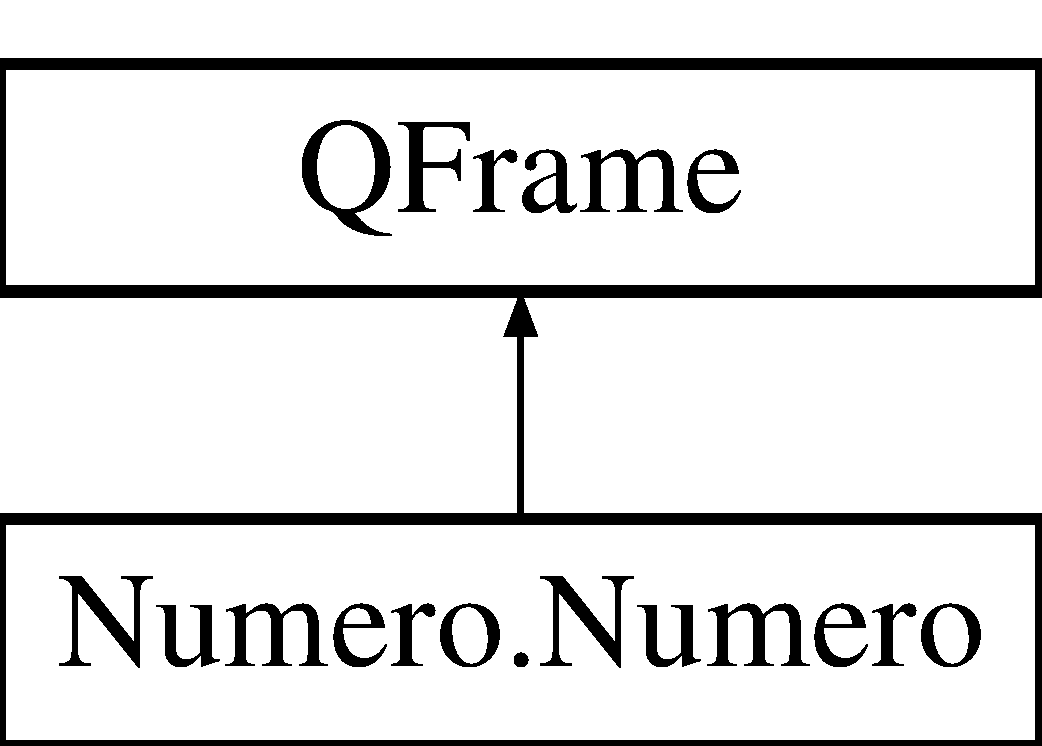
\includegraphics[height=2.000000cm]{class_numero_1_1_numero}
\end{center}
\end{figure}
\subsection*{Public Member Functions}
\begin{DoxyCompactItemize}
\item 
\hypertarget{class_numero_1_1_numero_a9f17c96d676757e0b155e88537e3abb3}{def {\bfseries \-\_\-\-\_\-init\-\_\-\-\_\-}}\label{class_numero_1_1_numero_a9f17c96d676757e0b155e88537e3abb3}

\item 
\hypertarget{class_numero_1_1_numero_a818d0986e959bc7475473acba2c9db52}{def {\bfseries set\-Numero}}\label{class_numero_1_1_numero_a818d0986e959bc7475473acba2c9db52}

\item 
\hypertarget{class_numero_1_1_numero_ae0fd65c2f86d7dd2bb094b35fcd85ab6}{def {\bfseries cambiar\-Color\-Boton\-Alerta}}\label{class_numero_1_1_numero_ae0fd65c2f86d7dd2bb094b35fcd85ab6}

\item 
\hypertarget{class_numero_1_1_numero_af740b535557fcd6bde1e43888e05a2fa}{def {\bfseries cambiar\-Color\-Boton\-Pista}}\label{class_numero_1_1_numero_af740b535557fcd6bde1e43888e05a2fa}

\item 
\hypertarget{class_numero_1_1_numero_ab1f9269d0aa574800961da32f7f95f16}{def {\bfseries cambiar\-Color\-Boton\-Original}}\label{class_numero_1_1_numero_ab1f9269d0aa574800961da32f7f95f16}

\item 
\hypertarget{class_numero_1_1_numero_a6ec5c677a3f7d8166aacf84b102eee0d}{def {\bfseries set\-Cuadricula}}\label{class_numero_1_1_numero_a6ec5c677a3f7d8166aacf84b102eee0d}

\end{DoxyCompactItemize}
\subsection*{Public Attributes}
\begin{DoxyCompactItemize}
\item 
\hypertarget{class_numero_1_1_numero_add58c510e6dfea0d3c3692c79e7c249a}{{\bfseries fila}}\label{class_numero_1_1_numero_add58c510e6dfea0d3c3692c79e7c249a}

\item 
\hypertarget{class_numero_1_1_numero_a4efc6e94fb89bf311c713fcda7fd7fac}{{\bfseries columna}}\label{class_numero_1_1_numero_a4efc6e94fb89bf311c713fcda7fd7fac}

\item 
\hypertarget{class_numero_1_1_numero_a9b4f5e3b0d3fa36ab48a1b25bc915b03}{{\bfseries valor\-Correcto}}\label{class_numero_1_1_numero_a9b4f5e3b0d3fa36ab48a1b25bc915b03}

\item 
\hypertarget{class_numero_1_1_numero_a79d57b9de0112d09194bff4aa2558fd8}{{\bfseries valor}}\label{class_numero_1_1_numero_a79d57b9de0112d09194bff4aa2558fd8}

\item 
\hypertarget{class_numero_1_1_numero_ab0d5b31bbf9e6ec1f8497bbf03ed68bf}{{\bfseries text\-Opciones}}\label{class_numero_1_1_numero_ab0d5b31bbf9e6ec1f8497bbf03ed68bf}

\item 
\hypertarget{class_numero_1_1_numero_aef53c5ef68a40f343af7a12d4fde21a0}{{\bfseries boton}}\label{class_numero_1_1_numero_aef53c5ef68a40f343af7a12d4fde21a0}

\item 
\hypertarget{class_numero_1_1_numero_a7a97cb3e4252e08aa77949a4aa616548}{{\bfseries cuadricula}}\label{class_numero_1_1_numero_a7a97cb3e4252e08aa77949a4aa616548}

\end{DoxyCompactItemize}
\subsection*{Static Public Attributes}
\begin{DoxyCompactItemize}
\item 
\hypertarget{class_numero_1_1_numero_a47b615282708c7153fce5360d06082ec}{int {\bfseries casilla} = -\/1}\label{class_numero_1_1_numero_a47b615282708c7153fce5360d06082ec}

\end{DoxyCompactItemize}


The documentation for this class was generated from the following file\-:\begin{DoxyCompactItemize}
\item 
C\-:/\-Users/\-Z\-A\-H\-I\-R  L\-U\-N\-A/\-Documents/\-Git\-Hub/\-Py\-Sudoku/ui/Numero.\-py\end{DoxyCompactItemize}

\hypertarget{class_sudoku_main_window_1_1_sudoku_main_window}{\section{Sudoku\-Main\-Window.\-Sudoku\-Main\-Window Class Reference}
\label{class_sudoku_main_window_1_1_sudoku_main_window}\index{Sudoku\-Main\-Window.\-Sudoku\-Main\-Window@{Sudoku\-Main\-Window.\-Sudoku\-Main\-Window}}
}
Inheritance diagram for Sudoku\-Main\-Window.\-Sudoku\-Main\-Window\-:\begin{figure}[H]
\begin{center}
\leavevmode
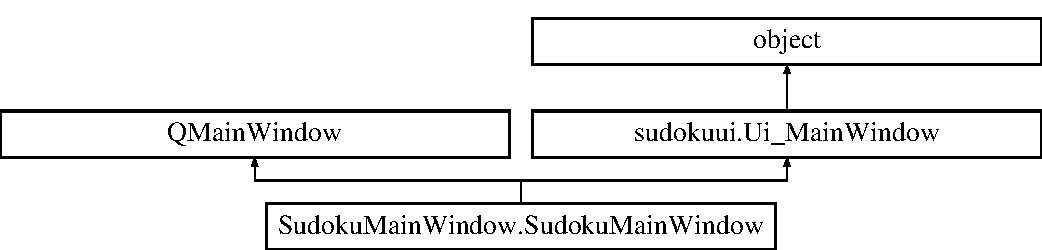
\includegraphics[height=3.000000cm]{class_sudoku_main_window_1_1_sudoku_main_window}
\end{center}
\end{figure}
\subsection*{Public Member Functions}
\begin{DoxyCompactItemize}
\item 
\hypertarget{class_sudoku_main_window_1_1_sudoku_main_window_a928fafad3bb263c11f16d84935cff2d2}{def {\bfseries \-\_\-\-\_\-init\-\_\-\-\_\-}}\label{class_sudoku_main_window_1_1_sudoku_main_window_a928fafad3bb263c11f16d84935cff2d2}

\item 
\hypertarget{class_sudoku_main_window_1_1_sudoku_main_window_adea80094a0be9e4f5cbde0c56713d64a}{def {\bfseries click\-Btn\-Llenar}}\label{class_sudoku_main_window_1_1_sudoku_main_window_adea80094a0be9e4f5cbde0c56713d64a}

\item 
\hypertarget{class_sudoku_main_window_1_1_sudoku_main_window_a3d717334d4dfec7d470cca6aca93055a}{def {\bfseries click\-Btn\-Finalizar}}\label{class_sudoku_main_window_1_1_sudoku_main_window_a3d717334d4dfec7d470cca6aca93055a}

\item 
\hypertarget{class_sudoku_main_window_1_1_sudoku_main_window_a52670b6c332989395bc5ea2e22b934a4}{def {\bfseries click\-Btn\-Ayuda}}\label{class_sudoku_main_window_1_1_sudoku_main_window_a52670b6c332989395bc5ea2e22b934a4}

\item 
\hypertarget{class_sudoku_main_window_1_1_sudoku_main_window_a998eec966a54bc105599f0b0da7c1c85}{def {\bfseries state\-Changed\-Chk\-Ayuda}}\label{class_sudoku_main_window_1_1_sudoku_main_window_a998eec966a54bc105599f0b0da7c1c85}

\item 
\hypertarget{class_sudoku_main_window_1_1_sudoku_main_window_ac8a0a4d664745d1e1d364051477cceab}{def {\bfseries state\-Changed\-Chk\-Alerta1}}\label{class_sudoku_main_window_1_1_sudoku_main_window_ac8a0a4d664745d1e1d364051477cceab}

\item 
\hypertarget{class_sudoku_main_window_1_1_sudoku_main_window_ac9eb37125e59154ae4a52d86dd4f950b}{def {\bfseries state\-Changed\-Chk\-Alerta2}}\label{class_sudoku_main_window_1_1_sudoku_main_window_ac9eb37125e59154ae4a52d86dd4f950b}

\item 
\hypertarget{class_sudoku_main_window_1_1_sudoku_main_window_a824e2abb8fae56fb9e1e717be893afb6}{def {\bfseries obtener\-Casilla}}\label{class_sudoku_main_window_1_1_sudoku_main_window_a824e2abb8fae56fb9e1e717be893afb6}

\item 
\hypertarget{class_sudoku_main_window_1_1_sudoku_main_window_ad2b406eb64afec77691ea9cb948e39fe}{def {\bfseries verificar\-Tablero\-Lleno}}\label{class_sudoku_main_window_1_1_sudoku_main_window_ad2b406eb64afec77691ea9cb948e39fe}

\item 
\hypertarget{class_sudoku_main_window_1_1_sudoku_main_window_a03974f85f3e539e3b25b4c6d1c153014}{def {\bfseries creacion\-Numeros}}\label{class_sudoku_main_window_1_1_sudoku_main_window_a03974f85f3e539e3b25b4c6d1c153014}

\item 
\hypertarget{class_sudoku_main_window_1_1_sudoku_main_window_a2f0494b5316de0f36057c788ee94bedf}{def {\bfseries creacion\-Botones}}\label{class_sudoku_main_window_1_1_sudoku_main_window_a2f0494b5316de0f36057c788ee94bedf}

\item 
\hypertarget{class_sudoku_main_window_1_1_sudoku_main_window_ad01ebfe88f98c98f9ae79759b2e842af}{def {\bfseries cambiar\-Numero}}\label{class_sudoku_main_window_1_1_sudoku_main_window_ad01ebfe88f98c98f9ae79759b2e842af}

\item 
\hypertarget{class_sudoku_main_window_1_1_sudoku_main_window_a06fd09150c43d8ed345473f78d15ae73}{def {\bfseries jugada\-Valida}}\label{class_sudoku_main_window_1_1_sudoku_main_window_a06fd09150c43d8ed345473f78d15ae73}

\item 
\hypertarget{class_sudoku_main_window_1_1_sudoku_main_window_a2ae3b41092df8aab696ea21ce4e3ae9c}{def {\bfseries jugada\-Correcta}}\label{class_sudoku_main_window_1_1_sudoku_main_window_a2ae3b41092df8aab696ea21ce4e3ae9c}

\item 
\hypertarget{class_sudoku_main_window_1_1_sudoku_main_window_aba7ba379fbf8b42dc8ff1e2a5884c4e9}{def {\bfseries color\-Original}}\label{class_sudoku_main_window_1_1_sudoku_main_window_aba7ba379fbf8b42dc8ff1e2a5884c4e9}

\item 
\hypertarget{class_sudoku_main_window_1_1_sudoku_main_window_a69afa66d148684c9ff528d44335670b8}{def {\bfseries color\-Invalidas}}\label{class_sudoku_main_window_1_1_sudoku_main_window_a69afa66d148684c9ff528d44335670b8}

\item 
\hypertarget{class_sudoku_main_window_1_1_sudoku_main_window_af769a5dcdde2c8b5a6edd70b77672960}{def {\bfseries color\-Incorrectas}}\label{class_sudoku_main_window_1_1_sudoku_main_window_af769a5dcdde2c8b5a6edd70b77672960}

\item 
\hypertarget{class_sudoku_main_window_1_1_sudoku_main_window_a54a131b93f52ac5dbd9c3ffcb8888b88}{def {\bfseries inicializar\-Timer}}\label{class_sudoku_main_window_1_1_sudoku_main_window_a54a131b93f52ac5dbd9c3ffcb8888b88}

\item 
\hypertarget{class_sudoku_main_window_1_1_sudoku_main_window_afbf8637004c9fae4db79d7e2beaf57c2}{def {\bfseries actualizar\-Timer}}\label{class_sudoku_main_window_1_1_sudoku_main_window_afbf8637004c9fae4db79d7e2beaf57c2}

\item 
\hypertarget{class_sudoku_main_window_1_1_sudoku_main_window_a1ccb72c504e09f04919e34418a846226}{def {\bfseries trigger\-Acerca\-De}}\label{class_sudoku_main_window_1_1_sudoku_main_window_a1ccb72c504e09f04919e34418a846226}

\item 
\hypertarget{class_sudoku_main_window_1_1_sudoku_main_window_a9d1f77df45624e15ebfcb58896a937fc}{def {\bfseries trigger\-Ayuda}}\label{class_sudoku_main_window_1_1_sudoku_main_window_a9d1f77df45624e15ebfcb58896a937fc}

\item 
\hypertarget{class_sudoku_main_window_1_1_sudoku_main_window_af8ad50f477151ecda2c6e76436ae00a3}{def {\bfseries trigger\-Mejores\-Tiempos}}\label{class_sudoku_main_window_1_1_sudoku_main_window_af8ad50f477151ecda2c6e76436ae00a3}

\item 
\hypertarget{class_sudoku_main_window_1_1_sudoku_main_window_afdfaf3e7d06aa50ec766fe212288fc29}{def {\bfseries trigger\-Guardar\-Partida}}\label{class_sudoku_main_window_1_1_sudoku_main_window_afdfaf3e7d06aa50ec766fe212288fc29}

\item 
\hypertarget{class_sudoku_main_window_1_1_sudoku_main_window_a9895205f897e2cd4e0552827253c74f9}{def {\bfseries trigger\-Cargar\-Partida}}\label{class_sudoku_main_window_1_1_sudoku_main_window_a9895205f897e2cd4e0552827253c74f9}

\item 
\hypertarget{class_sudoku_main_window_1_1_sudoku_main_window_a01b9c578d67e3b0cb0fb0836b204e2e3}{def {\bfseries tiempo\-Guardado}}\label{class_sudoku_main_window_1_1_sudoku_main_window_a01b9c578d67e3b0cb0fb0836b204e2e3}

\end{DoxyCompactItemize}
\subsection*{Public Attributes}
\begin{DoxyCompactItemize}
\item 
\hypertarget{class_sudoku_main_window_1_1_sudoku_main_window_ac2e9cceaaf36e4d4d0ffbd646dca0fd9}{{\bfseries numeros}}\label{class_sudoku_main_window_1_1_sudoku_main_window_ac2e9cceaaf36e4d4d0ffbd646dca0fd9}

\item 
\hypertarget{class_sudoku_main_window_1_1_sudoku_main_window_a012a36be9d3f9648a1c1f89649a8d259}{{\bfseries sgnl\-Mpr\-Numero}}\label{class_sudoku_main_window_1_1_sudoku_main_window_a012a36be9d3f9648a1c1f89649a8d259}

\item 
\hypertarget{class_sudoku_main_window_1_1_sudoku_main_window_a00f4ef9be740b78d47a6c8d99a102205}{{\bfseries sgnl\-Mpr\-Opcion}}\label{class_sudoku_main_window_1_1_sudoku_main_window_a00f4ef9be740b78d47a6c8d99a102205}

\item 
\hypertarget{class_sudoku_main_window_1_1_sudoku_main_window_a114dac730b306137fc13474cd9eabd8c}{{\bfseries casilla}}\label{class_sudoku_main_window_1_1_sudoku_main_window_a114dac730b306137fc13474cd9eabd8c}

\item 
\hypertarget{class_sudoku_main_window_1_1_sudoku_main_window_a2fd32e4e0d7e82a464ac3898ccc4637c}{{\bfseries color\-Cambiado}}\label{class_sudoku_main_window_1_1_sudoku_main_window_a2fd32e4e0d7e82a464ac3898ccc4637c}

\item 
\hypertarget{class_sudoku_main_window_1_1_sudoku_main_window_a645017ef826b404061c0954d702e81e1}{{\bfseries dificultad}}\label{class_sudoku_main_window_1_1_sudoku_main_window_a645017ef826b404061c0954d702e81e1}

\item 
\hypertarget{class_sudoku_main_window_1_1_sudoku_main_window_a3b5e5c8e03833814d82f4ca1531af9c2}{{\bfseries ayuda\-Usada}}\label{class_sudoku_main_window_1_1_sudoku_main_window_a3b5e5c8e03833814d82f4ca1531af9c2}

\item 
\hypertarget{class_sudoku_main_window_1_1_sudoku_main_window_afe8f983f779fc16f942e202865024b15}{{\bfseries tablero\-Lleno}}\label{class_sudoku_main_window_1_1_sudoku_main_window_afe8f983f779fc16f942e202865024b15}

\item 
\hypertarget{class_sudoku_main_window_1_1_sudoku_main_window_a549e0432a4386a67cb4ee4d3741c0835}{{\bfseries tablero\-Existe}}\label{class_sudoku_main_window_1_1_sudoku_main_window_a549e0432a4386a67cb4ee4d3741c0835}

\item 
\hypertarget{class_sudoku_main_window_1_1_sudoku_main_window_ade06c7abd46ed3d4385ebf0e01b670b1}{{\bfseries time\-Inicial}}\label{class_sudoku_main_window_1_1_sudoku_main_window_ade06c7abd46ed3d4385ebf0e01b670b1}

\item 
\hypertarget{class_sudoku_main_window_1_1_sudoku_main_window_ace319036ada7a045ab675ff38fa8ddb1}{{\bfseries timer}}\label{class_sudoku_main_window_1_1_sudoku_main_window_ace319036ada7a045ab675ff38fa8ddb1}

\item 
\hypertarget{class_sudoku_main_window_1_1_sudoku_main_window_ae9b4ab2489626295aa20808e8ffeeeca}{{\bfseries nombre}}\label{class_sudoku_main_window_1_1_sudoku_main_window_ae9b4ab2489626295aa20808e8ffeeeca}

\item 
\hypertarget{class_sudoku_main_window_1_1_sudoku_main_window_a370ea64e9453cab45cf57647f8ce6cf9}{{\bfseries opciones\-Numeros}}\label{class_sudoku_main_window_1_1_sudoku_main_window_a370ea64e9453cab45cf57647f8ce6cf9}

\item 
\hypertarget{class_sudoku_main_window_1_1_sudoku_main_window_a252168ae5d3f829d9403336f3c8893a3}{{\bfseries timer\-Texto}}\label{class_sudoku_main_window_1_1_sudoku_main_window_a252168ae5d3f829d9403336f3c8893a3}

\item 
\hypertarget{class_sudoku_main_window_1_1_sudoku_main_window_af4af3149f7ab37219efac57129609402}{{\bfseries timer\-Valor}}\label{class_sudoku_main_window_1_1_sudoku_main_window_af4af3149f7ab37219efac57129609402}

\end{DoxyCompactItemize}


\subsection{Detailed Description}
\begin{DoxyVerb}Metodo constructor
  Inicializa las variables usadas en la aplicacion e implementa las conexiones entre botones
  y la barra de menu.
\end{DoxyVerb}
 

The documentation for this class was generated from the following file\-:\begin{DoxyCompactItemize}
\item 
C\-:/\-Users/\-Z\-A\-H\-I\-R  L\-U\-N\-A/\-Documents/\-Git\-Hub/\-Py\-Sudoku/ui/Sudoku\-Main\-Window.\-py\end{DoxyCompactItemize}

\hypertarget{classacercade_u_i_1_1_ui___acerca_de}{\section{acercade\-U\-I.\-Ui\-\_\-\-Acerca\-De Class Reference}
\label{classacercade_u_i_1_1_ui___acerca_de}\index{acercade\-U\-I.\-Ui\-\_\-\-Acerca\-De@{acercade\-U\-I.\-Ui\-\_\-\-Acerca\-De}}
}
Inheritance diagram for acercade\-U\-I.\-Ui\-\_\-\-Acerca\-De\-:\begin{figure}[H]
\begin{center}
\leavevmode
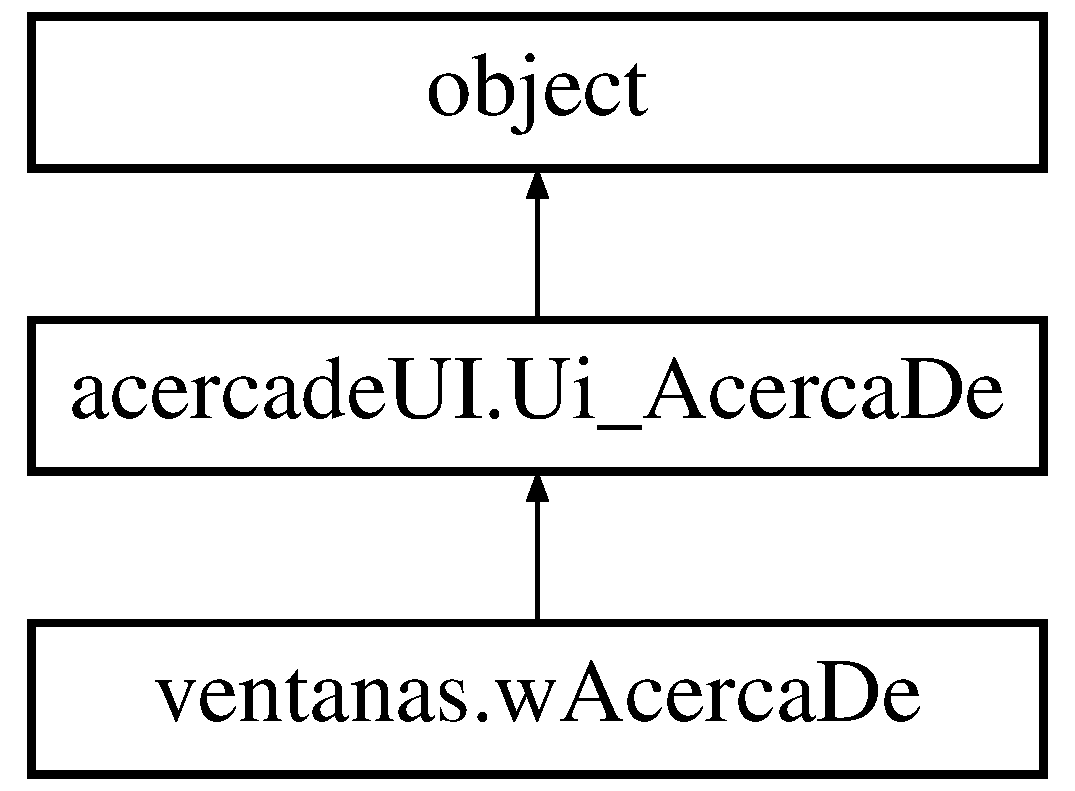
\includegraphics[height=3.000000cm]{classacercade_u_i_1_1_ui___acerca_de}
\end{center}
\end{figure}
\subsection*{Public Member Functions}
\begin{DoxyCompactItemize}
\item 
\hypertarget{classacercade_u_i_1_1_ui___acerca_de_aefd67a324d3a0f1b22deb4dc4e4a440d}{def {\bfseries setup\-Ui}}\label{classacercade_u_i_1_1_ui___acerca_de_aefd67a324d3a0f1b22deb4dc4e4a440d}

\item 
\hypertarget{classacercade_u_i_1_1_ui___acerca_de_a470228c7638375668f956cd52ac985ff}{def {\bfseries retranslate\-Ui}}\label{classacercade_u_i_1_1_ui___acerca_de_a470228c7638375668f956cd52ac985ff}

\end{DoxyCompactItemize}
\subsection*{Public Attributes}
\begin{DoxyCompactItemize}
\item 
\hypertarget{classacercade_u_i_1_1_ui___acerca_de_a867506749372d38d091f6f45ac68cdf5}{{\bfseries label\-\_\-2}}\label{classacercade_u_i_1_1_ui___acerca_de_a867506749372d38d091f6f45ac68cdf5}

\item 
\hypertarget{classacercade_u_i_1_1_ui___acerca_de_abb0b29b87b4861d692b65d2e6234b579}{{\bfseries label}}\label{classacercade_u_i_1_1_ui___acerca_de_abb0b29b87b4861d692b65d2e6234b579}

\end{DoxyCompactItemize}


The documentation for this class was generated from the following file\-:\begin{DoxyCompactItemize}
\item 
C\-:/\-Users/\-Z\-A\-H\-I\-R  L\-U\-N\-A/\-Documents/\-Git\-Hub/\-Py\-Sudoku/ui/acercade\-U\-I.\-py\end{DoxyCompactItemize}

\hypertarget{classayuda_u_i_1_1_ui___ayuda}{\section{ayuda\-U\-I.\-Ui\-\_\-\-Ayuda Class Reference}
\label{classayuda_u_i_1_1_ui___ayuda}\index{ayuda\-U\-I.\-Ui\-\_\-\-Ayuda@{ayuda\-U\-I.\-Ui\-\_\-\-Ayuda}}
}
Inheritance diagram for ayuda\-U\-I.\-Ui\-\_\-\-Ayuda\-:\begin{figure}[H]
\begin{center}
\leavevmode
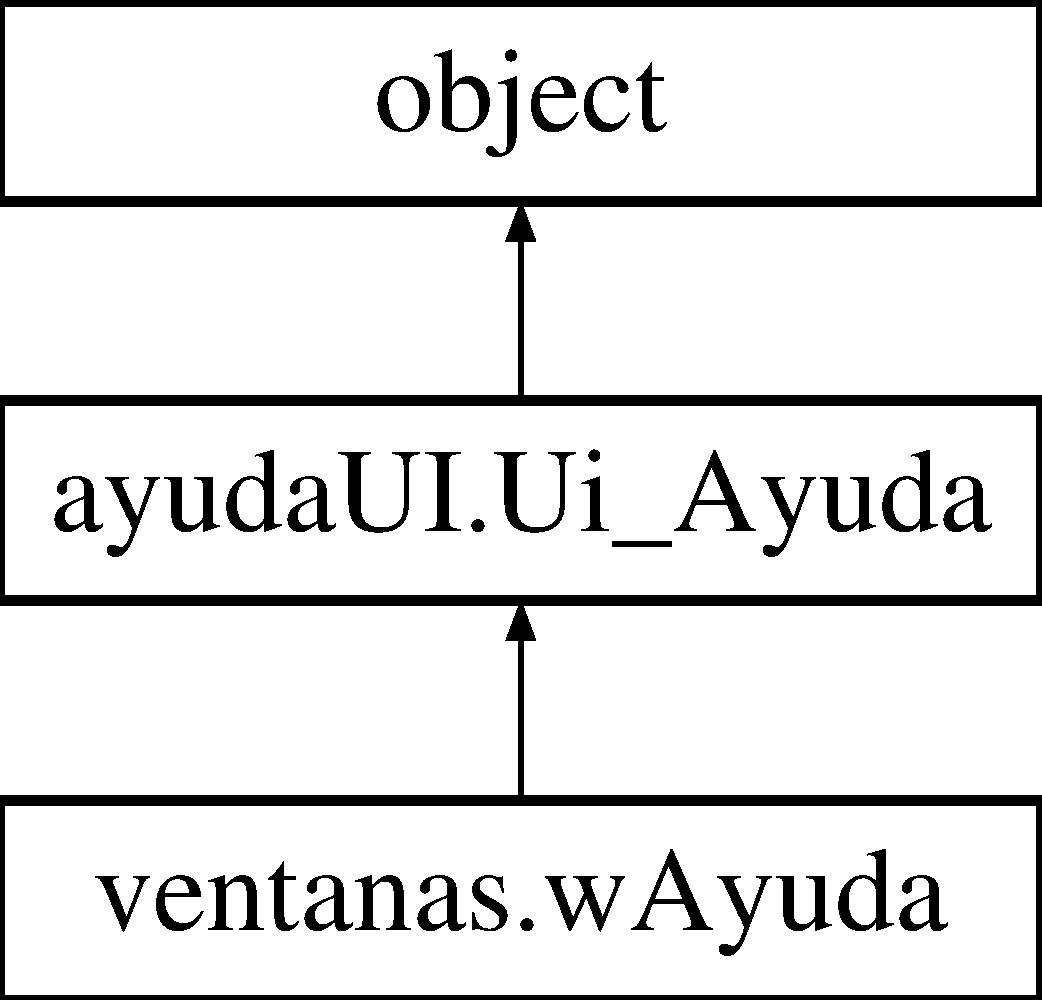
\includegraphics[height=3.000000cm]{classayuda_u_i_1_1_ui___ayuda}
\end{center}
\end{figure}
\subsection*{Public Member Functions}
\begin{DoxyCompactItemize}
\item 
\hypertarget{classayuda_u_i_1_1_ui___ayuda_a616863ea29f44f7f52d368e09f480753}{def {\bfseries setup\-Ui}}\label{classayuda_u_i_1_1_ui___ayuda_a616863ea29f44f7f52d368e09f480753}

\item 
\hypertarget{classayuda_u_i_1_1_ui___ayuda_a9eff96f141f61c51614d817a9a0f16a7}{def {\bfseries retranslate\-Ui}}\label{classayuda_u_i_1_1_ui___ayuda_a9eff96f141f61c51614d817a9a0f16a7}

\end{DoxyCompactItemize}
\subsection*{Public Attributes}
\begin{DoxyCompactItemize}
\item 
\hypertarget{classayuda_u_i_1_1_ui___ayuda_a2b56f75a292ff08c862a23b55b60525c}{{\bfseries label}}\label{classayuda_u_i_1_1_ui___ayuda_a2b56f75a292ff08c862a23b55b60525c}

\item 
\hypertarget{classayuda_u_i_1_1_ui___ayuda_afe089ef2b986a612644064f9a178c3c5}{{\bfseries label\-\_\-2}}\label{classayuda_u_i_1_1_ui___ayuda_afe089ef2b986a612644064f9a178c3c5}

\item 
\hypertarget{classayuda_u_i_1_1_ui___ayuda_ac4a0b3f55d0bd9996436e79857e8e8d9}{{\bfseries push\-Button}}\label{classayuda_u_i_1_1_ui___ayuda_ac4a0b3f55d0bd9996436e79857e8e8d9}

\end{DoxyCompactItemize}


The documentation for this class was generated from the following file\-:\begin{DoxyCompactItemize}
\item 
C\-:/\-Users/\-Z\-A\-H\-I\-R  L\-U\-N\-A/\-Documents/\-Git\-Hub/\-Py\-Sudoku/ui/ayuda\-U\-I.\-py\end{DoxyCompactItemize}

\hypertarget{classsudokuui_1_1_ui___main_window}{\section{sudokuui.\-Ui\-\_\-\-Main\-Window Class Reference}
\label{classsudokuui_1_1_ui___main_window}\index{sudokuui.\-Ui\-\_\-\-Main\-Window@{sudokuui.\-Ui\-\_\-\-Main\-Window}}
}
Inheritance diagram for sudokuui.\-Ui\-\_\-\-Main\-Window\-:\begin{figure}[H]
\begin{center}
\leavevmode
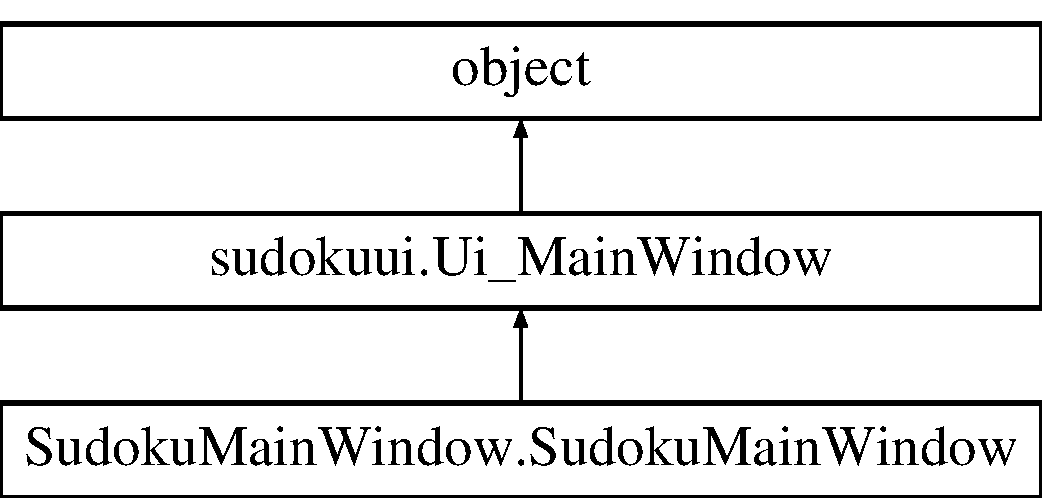
\includegraphics[height=3.000000cm]{classsudokuui_1_1_ui___main_window}
\end{center}
\end{figure}
\subsection*{Public Member Functions}
\begin{DoxyCompactItemize}
\item 
\hypertarget{classsudokuui_1_1_ui___main_window_af7d8582f64fe04816c4ea928b3601f9a}{def {\bfseries setup\-Ui}}\label{classsudokuui_1_1_ui___main_window_af7d8582f64fe04816c4ea928b3601f9a}

\item 
\hypertarget{classsudokuui_1_1_ui___main_window_a757ddd14ff06b39edc0d04a4d7e10a57}{def {\bfseries retranslate\-Ui}}\label{classsudokuui_1_1_ui___main_window_a757ddd14ff06b39edc0d04a4d7e10a57}

\end{DoxyCompactItemize}
\subsection*{Public Attributes}
\begin{DoxyCompactItemize}
\item 
\hypertarget{classsudokuui_1_1_ui___main_window_a6282b23abd869a67f2c219780778a8c6}{{\bfseries central\-Widget}}\label{classsudokuui_1_1_ui___main_window_a6282b23abd869a67f2c219780778a8c6}

\item 
\hypertarget{classsudokuui_1_1_ui___main_window_a6114e11c94c892dcf77dd23789f51699}{{\bfseries grid\-Layout\-Widget}}\label{classsudokuui_1_1_ui___main_window_a6114e11c94c892dcf77dd23789f51699}

\item 
\hypertarget{classsudokuui_1_1_ui___main_window_a53f586e421a5620c8266427717d65c5a}{{\bfseries grid\-Tablero}}\label{classsudokuui_1_1_ui___main_window_a53f586e421a5620c8266427717d65c5a}

\item 
\hypertarget{classsudokuui_1_1_ui___main_window_ad26c91c6900eab0caf64c40bcc65f630}{{\bfseries label}}\label{classsudokuui_1_1_ui___main_window_ad26c91c6900eab0caf64c40bcc65f630}

\item 
\hypertarget{classsudokuui_1_1_ui___main_window_ad670263c469deb42388573cab852bbcb}{{\bfseries gb\-Opciones}}\label{classsudokuui_1_1_ui___main_window_ad670263c469deb42388573cab852bbcb}

\item 
\hypertarget{classsudokuui_1_1_ui___main_window_a8aa7947d3bd7e9face48a26d107f0aff}{{\bfseries chk\-Alerta1}}\label{classsudokuui_1_1_ui___main_window_a8aa7947d3bd7e9face48a26d107f0aff}

\item 
\hypertarget{classsudokuui_1_1_ui___main_window_a6dd6f7f93cf5c4505bdfe48dc93440d1}{{\bfseries chk\-Alerta2}}\label{classsudokuui_1_1_ui___main_window_a6dd6f7f93cf5c4505bdfe48dc93440d1}

\item 
\hypertarget{classsudokuui_1_1_ui___main_window_a872ae8b9cd92af2bf64744c768cb7235}{{\bfseries chk\-Ayuda}}\label{classsudokuui_1_1_ui___main_window_a872ae8b9cd92af2bf64744c768cb7235}

\item 
\hypertarget{classsudokuui_1_1_ui___main_window_adde0a7697330b695f90441f33def153c}{{\bfseries chk\-Pista}}\label{classsudokuui_1_1_ui___main_window_adde0a7697330b695f90441f33def153c}

\item 
\hypertarget{classsudokuui_1_1_ui___main_window_afe2dd318a5271ae1ea045c32cf82f931}{{\bfseries btn\-Llenar}}\label{classsudokuui_1_1_ui___main_window_afe2dd318a5271ae1ea045c32cf82f931}

\item 
\hypertarget{classsudokuui_1_1_ui___main_window_a6e9dc327440fb1404a0dd6ddb393ac55}{{\bfseries gb\-Numeros}}\label{classsudokuui_1_1_ui___main_window_a6e9dc327440fb1404a0dd6ddb393ac55}

\item 
\hypertarget{classsudokuui_1_1_ui___main_window_aff24a3956daf91fb973908fb3400c886}{{\bfseries grid\-Layout\-Widget\-\_\-2}}\label{classsudokuui_1_1_ui___main_window_aff24a3956daf91fb973908fb3400c886}

\item 
\hypertarget{classsudokuui_1_1_ui___main_window_a72c2a396c49ba9923f65bee3b2cff122}{{\bfseries grid\-Numeros}}\label{classsudokuui_1_1_ui___main_window_a72c2a396c49ba9923f65bee3b2cff122}

\item 
\hypertarget{classsudokuui_1_1_ui___main_window_af04c8ff967d04e7b7b63fa6bc6beb462}{{\bfseries btn\-Ayuda}}\label{classsudokuui_1_1_ui___main_window_af04c8ff967d04e7b7b63fa6bc6beb462}

\item 
\hypertarget{classsudokuui_1_1_ui___main_window_a905a485955cc4100e693759f088ef606}{{\bfseries lcd\-Number}}\label{classsudokuui_1_1_ui___main_window_a905a485955cc4100e693759f088ef606}

\item 
\hypertarget{classsudokuui_1_1_ui___main_window_a58e053292b250741df9883947b3681b6}{{\bfseries btn\-Finalizar}}\label{classsudokuui_1_1_ui___main_window_a58e053292b250741df9883947b3681b6}

\item 
\hypertarget{classsudokuui_1_1_ui___main_window_a886be2c8e87819b286060f8a47926f5b}{{\bfseries layout\-Widget}}\label{classsudokuui_1_1_ui___main_window_a886be2c8e87819b286060f8a47926f5b}

\item 
\hypertarget{classsudokuui_1_1_ui___main_window_a9655e75db8ffee6fce920fa812f98b4f}{{\bfseries horizontal\-Layout}}\label{classsudokuui_1_1_ui___main_window_a9655e75db8ffee6fce920fa812f98b4f}

\item 
\hypertarget{classsudokuui_1_1_ui___main_window_a123c28199b8cdba685b8a0022b7f8875}{{\bfseries lbl\-Dificultad}}\label{classsudokuui_1_1_ui___main_window_a123c28199b8cdba685b8a0022b7f8875}

\item 
\hypertarget{classsudokuui_1_1_ui___main_window_abe7885f4b93b68e82746d821d4ba9923}{{\bfseries cbo\-Dificultad}}\label{classsudokuui_1_1_ui___main_window_abe7885f4b93b68e82746d821d4ba9923}

\item 
\hypertarget{classsudokuui_1_1_ui___main_window_a9f5b2d7c8eee38437345d5f0462470dd}{{\bfseries menu\-Bar}}\label{classsudokuui_1_1_ui___main_window_a9f5b2d7c8eee38437345d5f0462470dd}

\item 
\hypertarget{classsudokuui_1_1_ui___main_window_a819f425769527ecb41842b727c15fd1f}{{\bfseries menu\-Menu}}\label{classsudokuui_1_1_ui___main_window_a819f425769527ecb41842b727c15fd1f}

\item 
\hypertarget{classsudokuui_1_1_ui___main_window_a24fb10bfd9502bdb77c073e738ef18e0}{{\bfseries menu\-Ayuda}}\label{classsudokuui_1_1_ui___main_window_a24fb10bfd9502bdb77c073e738ef18e0}

\item 
\hypertarget{classsudokuui_1_1_ui___main_window_a89e552c24ec54060de22f7b30664c31f}{{\bfseries main\-Tool\-Bar}}\label{classsudokuui_1_1_ui___main_window_a89e552c24ec54060de22f7b30664c31f}

\item 
\hypertarget{classsudokuui_1_1_ui___main_window_ac5a84bcb1c39736fbac28f62d6f3fc28}{{\bfseries action\-Nueva\-\_\-partida}}\label{classsudokuui_1_1_ui___main_window_ac5a84bcb1c39736fbac28f62d6f3fc28}

\item 
\hypertarget{classsudokuui_1_1_ui___main_window_a4e095dc0bbf558facc5b1e62cc325ff4}{{\bfseries action\-Guardar\-\_\-partida}}\label{classsudokuui_1_1_ui___main_window_a4e095dc0bbf558facc5b1e62cc325ff4}

\item 
\hypertarget{classsudokuui_1_1_ui___main_window_a78dd95829203c345bcc2f41743348f57}{{\bfseries action\-Cargar\-\_\-partida}}\label{classsudokuui_1_1_ui___main_window_a78dd95829203c345bcc2f41743348f57}

\item 
\hypertarget{classsudokuui_1_1_ui___main_window_acf580ed577baa24a3052ca3784cde3d0}{{\bfseries action\-Salir}}\label{classsudokuui_1_1_ui___main_window_acf580ed577baa24a3052ca3784cde3d0}

\item 
\hypertarget{classsudokuui_1_1_ui___main_window_a727fd47e605aba698f3ccd7fdef2b559}{{\bfseries action\-Ayuda}}\label{classsudokuui_1_1_ui___main_window_a727fd47e605aba698f3ccd7fdef2b559}

\item 
\hypertarget{classsudokuui_1_1_ui___main_window_a2e0a25588fa107e4c61181ed80bb3a46}{{\bfseries action\-Acerca\-\_\-de}}\label{classsudokuui_1_1_ui___main_window_a2e0a25588fa107e4c61181ed80bb3a46}

\item 
\hypertarget{classsudokuui_1_1_ui___main_window_aece3a743957be27f6f09c6c882582958}{{\bfseries action\-Mejores\-\_\-tiempos}}\label{classsudokuui_1_1_ui___main_window_aece3a743957be27f6f09c6c882582958}

\end{DoxyCompactItemize}


The documentation for this class was generated from the following file\-:\begin{DoxyCompactItemize}
\item 
C\-:/\-Users/\-Z\-A\-H\-I\-R  L\-U\-N\-A/\-Documents/\-Git\-Hub/\-Py\-Sudoku/ui/sudokuui.\-py\end{DoxyCompactItemize}

\hypertarget{classmejores_tiempos_u_i_1_1_ui___mejores_tiempos}{\section{mejores\-Tiempos\-U\-I.\-Ui\-\_\-\-Mejores\-Tiempos Class Reference}
\label{classmejores_tiempos_u_i_1_1_ui___mejores_tiempos}\index{mejores\-Tiempos\-U\-I.\-Ui\-\_\-\-Mejores\-Tiempos@{mejores\-Tiempos\-U\-I.\-Ui\-\_\-\-Mejores\-Tiempos}}
}
Inheritance diagram for mejores\-Tiempos\-U\-I.\-Ui\-\_\-\-Mejores\-Tiempos\-:\begin{figure}[H]
\begin{center}
\leavevmode
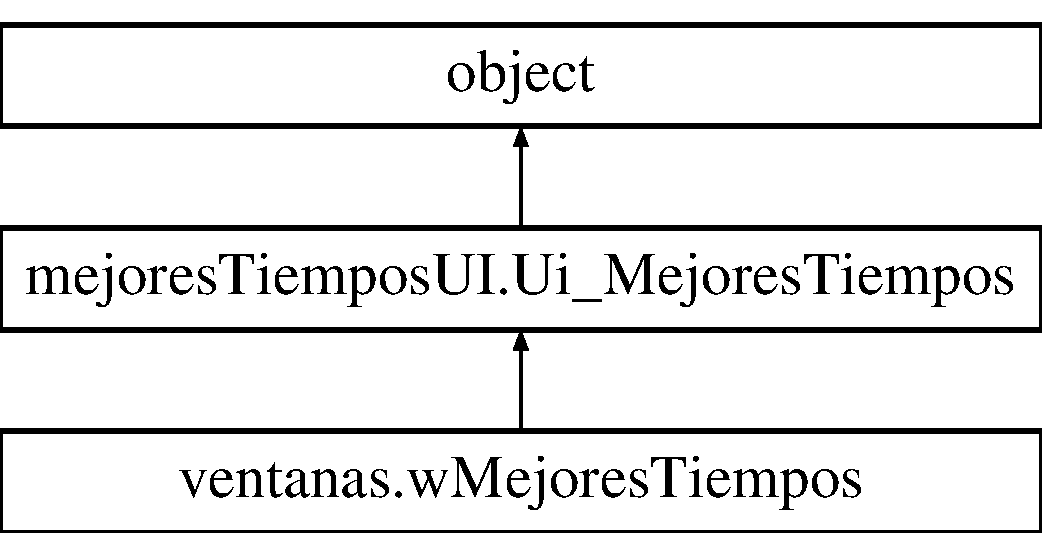
\includegraphics[height=3.000000cm]{classmejores_tiempos_u_i_1_1_ui___mejores_tiempos}
\end{center}
\end{figure}
\subsection*{Public Member Functions}
\begin{DoxyCompactItemize}
\item 
\hypertarget{classmejores_tiempos_u_i_1_1_ui___mejores_tiempos_a6bb0f6b347b6fd5c57628191ef6e454e}{def {\bfseries setup\-Ui}}\label{classmejores_tiempos_u_i_1_1_ui___mejores_tiempos_a6bb0f6b347b6fd5c57628191ef6e454e}

\item 
\hypertarget{classmejores_tiempos_u_i_1_1_ui___mejores_tiempos_a6635519238cb6b3fa06d8251cb802204}{def {\bfseries retranslate\-Ui}}\label{classmejores_tiempos_u_i_1_1_ui___mejores_tiempos_a6635519238cb6b3fa06d8251cb802204}

\end{DoxyCompactItemize}
\subsection*{Public Attributes}
\begin{DoxyCompactItemize}
\item 
\hypertarget{classmejores_tiempos_u_i_1_1_ui___mejores_tiempos_aa8cd68c61a7f36c8e6cc03089279d252}{{\bfseries tab}}\label{classmejores_tiempos_u_i_1_1_ui___mejores_tiempos_aa8cd68c61a7f36c8e6cc03089279d252}

\item 
\hypertarget{classmejores_tiempos_u_i_1_1_ui___mejores_tiempos_a1f9270a09ec22df65af2c88f22272d2d}{{\bfseries tab\-Principiante}}\label{classmejores_tiempos_u_i_1_1_ui___mejores_tiempos_a1f9270a09ec22df65af2c88f22272d2d}

\item 
\hypertarget{classmejores_tiempos_u_i_1_1_ui___mejores_tiempos_abc7def506bcb43a74f16e2d3f42b44a2}{{\bfseries table\-Principiante}}\label{classmejores_tiempos_u_i_1_1_ui___mejores_tiempos_abc7def506bcb43a74f16e2d3f42b44a2}

\item 
\hypertarget{classmejores_tiempos_u_i_1_1_ui___mejores_tiempos_a5ba8a8ab05843d64b9d940d436351ce3}{{\bfseries tab\-Intermedio}}\label{classmejores_tiempos_u_i_1_1_ui___mejores_tiempos_a5ba8a8ab05843d64b9d940d436351ce3}

\item 
\hypertarget{classmejores_tiempos_u_i_1_1_ui___mejores_tiempos_a5c7d5b9816496271ee8f575407f62074}{{\bfseries table\-Intermedio}}\label{classmejores_tiempos_u_i_1_1_ui___mejores_tiempos_a5c7d5b9816496271ee8f575407f62074}

\item 
\hypertarget{classmejores_tiempos_u_i_1_1_ui___mejores_tiempos_a96e6b62d20314aa8135213e1b682be27}{{\bfseries tab\-Avanzado}}\label{classmejores_tiempos_u_i_1_1_ui___mejores_tiempos_a96e6b62d20314aa8135213e1b682be27}

\item 
\hypertarget{classmejores_tiempos_u_i_1_1_ui___mejores_tiempos_ae5921b387d85a354e084cc4e631eee06}{{\bfseries table\-Avanzado}}\label{classmejores_tiempos_u_i_1_1_ui___mejores_tiempos_ae5921b387d85a354e084cc4e631eee06}

\item 
\hypertarget{classmejores_tiempos_u_i_1_1_ui___mejores_tiempos_a83fa8701e748d74c24954570349860cd}{{\bfseries label\-Mejores\-Tiempos}}\label{classmejores_tiempos_u_i_1_1_ui___mejores_tiempos_a83fa8701e748d74c24954570349860cd}

\item 
\hypertarget{classmejores_tiempos_u_i_1_1_ui___mejores_tiempos_ae8e938354726bd2ac50902586b157505}{{\bfseries push\-Button}}\label{classmejores_tiempos_u_i_1_1_ui___mejores_tiempos_ae8e938354726bd2ac50902586b157505}

\end{DoxyCompactItemize}


The documentation for this class was generated from the following file\-:\begin{DoxyCompactItemize}
\item 
C\-:/\-Users/\-Z\-A\-H\-I\-R  L\-U\-N\-A/\-Documents/\-Git\-Hub/\-Py\-Sudoku/ui/mejores\-Tiempos\-U\-I.\-py\end{DoxyCompactItemize}

\hypertarget{classventanas_1_1w_acerca_de}{\section{ventanas.\-w\-Acerca\-De Class Reference}
\label{classventanas_1_1w_acerca_de}\index{ventanas.\-w\-Acerca\-De@{ventanas.\-w\-Acerca\-De}}
}
Inheritance diagram for ventanas.\-w\-Acerca\-De\-:\begin{figure}[H]
\begin{center}
\leavevmode
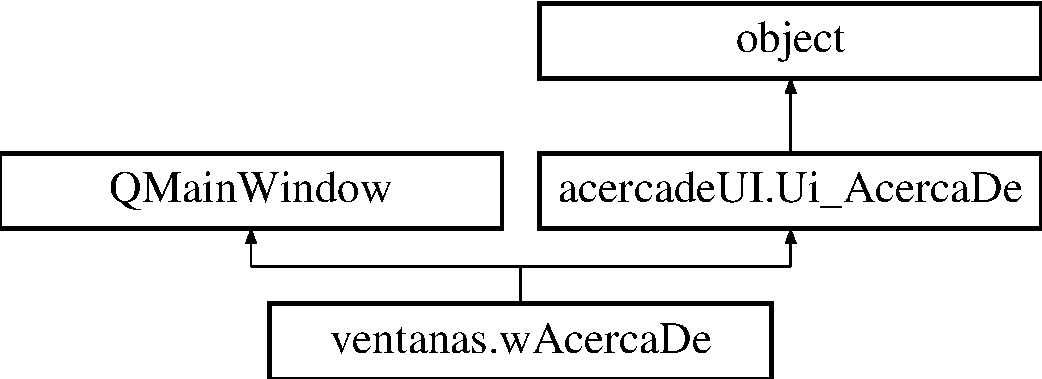
\includegraphics[height=3.000000cm]{classventanas_1_1w_acerca_de}
\end{center}
\end{figure}
\subsection*{Public Member Functions}
\begin{DoxyCompactItemize}
\item 
\hypertarget{classventanas_1_1w_acerca_de_ab18d9b92c4620ef50d91072e7d17eee3}{def {\bfseries \-\_\-\-\_\-init\-\_\-\-\_\-}}\label{classventanas_1_1w_acerca_de_ab18d9b92c4620ef50d91072e7d17eee3}

\end{DoxyCompactItemize}
\subsection*{Additional Inherited Members}


The documentation for this class was generated from the following file\-:\begin{DoxyCompactItemize}
\item 
C\-:/\-Users/\-Z\-A\-H\-I\-R  L\-U\-N\-A/\-Documents/\-Git\-Hub/\-Py\-Sudoku/ui/ventanas.\-py\end{DoxyCompactItemize}

\hypertarget{classventanas_1_1w_ayuda}{\section{ventanas.\-w\-Ayuda Class Reference}
\label{classventanas_1_1w_ayuda}\index{ventanas.\-w\-Ayuda@{ventanas.\-w\-Ayuda}}
}
Inheritance diagram for ventanas.\-w\-Ayuda\-:\begin{figure}[H]
\begin{center}
\leavevmode
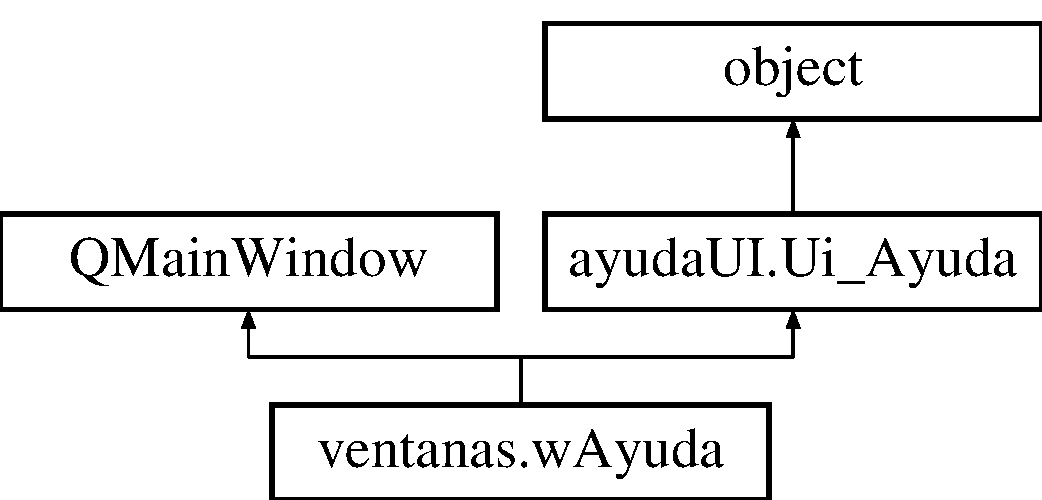
\includegraphics[height=3.000000cm]{classventanas_1_1w_ayuda}
\end{center}
\end{figure}
\subsection*{Public Member Functions}
\begin{DoxyCompactItemize}
\item 
\hypertarget{classventanas_1_1w_ayuda_a75ddc112e68887106f7964a7788f5d90}{def {\bfseries \-\_\-\-\_\-init\-\_\-\-\_\-}}\label{classventanas_1_1w_ayuda_a75ddc112e68887106f7964a7788f5d90}

\end{DoxyCompactItemize}
\subsection*{Additional Inherited Members}


The documentation for this class was generated from the following file\-:\begin{DoxyCompactItemize}
\item 
C\-:/\-Users/\-Z\-A\-H\-I\-R  L\-U\-N\-A/\-Documents/\-Git\-Hub/\-Py\-Sudoku/ui/ventanas.\-py\end{DoxyCompactItemize}

\hypertarget{classventanas_1_1w_mejores_tiempos}{\section{ventanas.\-w\-Mejores\-Tiempos Class Reference}
\label{classventanas_1_1w_mejores_tiempos}\index{ventanas.\-w\-Mejores\-Tiempos@{ventanas.\-w\-Mejores\-Tiempos}}
}
Inheritance diagram for ventanas.\-w\-Mejores\-Tiempos\-:\begin{figure}[H]
\begin{center}
\leavevmode
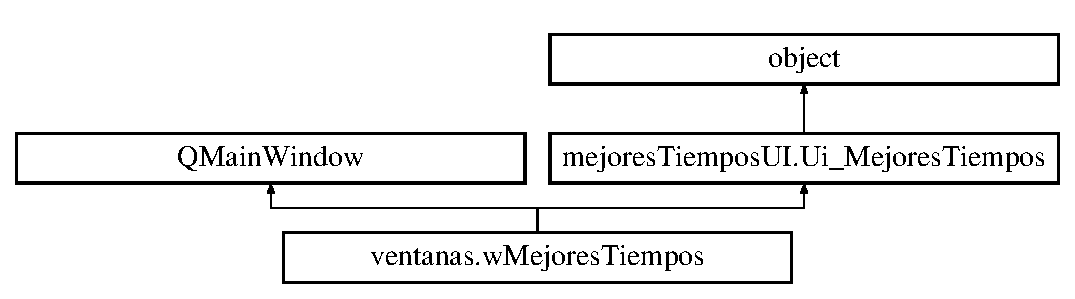
\includegraphics[height=3.000000cm]{classventanas_1_1w_mejores_tiempos}
\end{center}
\end{figure}
\subsection*{Public Member Functions}
\begin{DoxyCompactItemize}
\item 
\hypertarget{classventanas_1_1w_mejores_tiempos_a9144362cf6259852285fdf4b0f7ab39b}{def {\bfseries \-\_\-\-\_\-init\-\_\-\-\_\-}}\label{classventanas_1_1w_mejores_tiempos_a9144362cf6259852285fdf4b0f7ab39b}

\item 
\hypertarget{classventanas_1_1w_mejores_tiempos_a1d1586af2cb7d6e4b16fc14b963a7b33}{def {\bfseries click\-Btn\-Salir}}\label{classventanas_1_1w_mejores_tiempos_a1d1586af2cb7d6e4b16fc14b963a7b33}

\item 
\hypertarget{classventanas_1_1w_mejores_tiempos_a4a22501803f7b0dfef0fae412d16eddd}{def {\bfseries guardar\-Tiempos}}\label{classventanas_1_1w_mejores_tiempos_a4a22501803f7b0dfef0fae412d16eddd}

\item 
\hypertarget{classventanas_1_1w_mejores_tiempos_a913d4d800d0492c403cf5668646ee629}{def {\bfseries cargar\-Tiempos}}\label{classventanas_1_1w_mejores_tiempos_a913d4d800d0492c403cf5668646ee629}

\item 
\hypertarget{classventanas_1_1w_mejores_tiempos_a7a3c86fec7473b1b05266a69bb418a9a}{def {\bfseries mostrar\-Tiempos}}\label{classventanas_1_1w_mejores_tiempos_a7a3c86fec7473b1b05266a69bb418a9a}

\end{DoxyCompactItemize}
\subsection*{Additional Inherited Members}


The documentation for this class was generated from the following file\-:\begin{DoxyCompactItemize}
\item 
C\-:/\-Users/\-Z\-A\-H\-I\-R  L\-U\-N\-A/\-Documents/\-Git\-Hub/\-Py\-Sudoku/ui/ventanas.\-py\end{DoxyCompactItemize}

%--- End generated contents ---

% Index
\newpage
\phantomsection
\addcontentsline{toc}{part}{Index}
\printindex

\end{document}
